\chapter{Cosmografia}
\label{cha:cosmografia}

\section[Introduzione]{Introduzione\footnote{In questo paragrafo introduttivo
    alla Cosmologia ho seguito gli appunti del corso di Cosmologia di
    A. Cavaliere, Università di Roma.}}

L'inizio della Cosmologia moderna può essere datato agli anni '20 del secolo
scorso con la scoperta di stelle variabili periodiche del tipo delle Cefeidi in
alcune nebulose a spirale tra cui M31 nella costellazione di Andromeda.  Poiché
era nota per le Cefeidi una relazione empirica tra periodo $P$ e luminosità
assoluta $L$, la distanza $D$ di M31 è determinata attraverso la misura del
flusso $F$ e l'utilizzo della relazione (valida nel caso euclideo)
\begin{equation}
  D=\left( \frac{L}{4 \pi F} \right)^{1/2}
\end{equation}
La distanza di M31 risultò\footnote{Tale distanza risultò in seguito errata per
  difetto a causa di una sottostima di $L$ --- dovuta all'aver trascurato
  l'assorbimento della luce da parte del mezzo interstellare (ISM).  Oggi noi
  sappiamo che la distanza di M31 è 770 kpc.} di circa 240 kpc (1 pc equivale a
$3.08 \times 10^{18}$ cm $\equiv 3.3$ anni luce) e pertanto molto maggiore delle
dimensioni visibili della nostra galassia (la Galassia o Via Lattea) che allora
erano stimate in 10 kpc, dimostrando in modo conclusivo che M31 costituiva un
intero sistema di stelle esterno alla Galassia.

La scoperta, comunicata da E. Hubble il 1 gennaio 1925, pose fine a una lunga
controversia tra gli astronomi sulla natura delle nebulose che furono
interpretate definitivamente come sistemi di stelle (universi isola) analoghi
alla Galassia.

È da sottolineare subito che le osservazioni astronomiche hanno la seguente
peculiarità.  A causa della velocità finita di propagazione della luce, quando
noi guardiamo lontano nello spazio, necessariamente guardiamo indietro nel tempo
e alla distanza $D$ corrisponde il tempo nel passato
\begin{equation}
  \Delta T = \frac{D}{c}
\end{equation}
per cui noi vediamo M31, la più vicina tra le grandi galassie a spirale simili
alla Galassia, come era 2.5 milioni di anni fa.

Noi viviamo in una Galassia a spirale tipica, di cui il Sole è una stella media
tra le circa $\simeq 3 \times 10^{11}$ che la compongono.  La luminosità
complessiva della Galassia è $L_G \simeq 2 \times 10^{10} L_{\odot}$ (la
luminosit solare è $L_{\odot} = 3.90 \times 10^{33}$ erg s$^{-1}$), mentre la
massa della Galassia è $M_G \simeq 10^{11} M_{\odot}$.

La densità media della Galassia, considerando gli atomi componenti le stelle e
una modesta quantità di gas interstellare uniformemente diffusi all'interno
della Galassia, è $\rho_G \simeq 10^{-23}$ g cm$^{-3}$, corrispondente a circa 5
atomi di idrogeno al cm$^{3}$.  È questa una densità estremamente bassa se
confrontata, ad esempio, con quella dell'aria.  Tuttavia, a causa delle enormi
dimensioni, essa è sufficiente a fare della Galassia un sistema isolato
auto-gravitante in cui le forze gravitazionali interne sono in equilibrio con i
moti delle stelle.

La Galassia è circondata in ogni sua parte, in media uniformemente, da altre
``isole di stelle'' (galassie) e la separazione media delle galassie è circa 3
Mpc.

In realtà vi è una netta tendenza delle galassie a formare gruppi, a loro volta
autogravitanti, di varia consistenza: da sistemi binari, a gruppi di poche
decine di galassie\footnote{La Galassia fa parte del Gruppo Locale costituito da
  25 galassie, delle quali M31 è la più grande e la Galassia è seconda per
  dimensioni.} fino agli ammassi composti da migliaia di galassie come, ad
esempio, Coma e Virgo, a distanza di circa 20 Mpc.

In sostanza, la materia tende a condensarsi su scale di dimensioni crescenti:
\begin{itemize}
\item il gas $\to$ stelle (di dimensioni $R_{\odot} \simeq 10^6$ km)
\item le stelle $\to$ galassie (di dimensioni fino a $R_G \simeq$ 100 kpc)
\item le galassie $\to$ gruppi o ammassi (di dimensioni fino a $R_{Cl}\simeq 3-10$ Mpc)
\item gli ammassi $\to$ super-ammassi (di dimensioni $\simeq$ 50 Mpc)
\end{itemize}
Questi ultimi non sono sistemi in equilibrio gravitazionale ben isolati e
appaiono prevalentemente contigui.  Le condensazioni di dimensioni
progressivamente maggiori hanno densità via via minori, mentre aumenta
fortemente il fattore di riempimento, cioè il rapporto tra il volume occupato
dai componenti ed il volume totale del sistema: le stelle riempiono solo una
frazione minuscola del volume delle galassie (la distanza media tra le stelle è
circa 1 pc) mentre i super-ammassi sono contigui.

La gerarchia di condensazioni termina con i super-ammassi e a dimensioni
superiori a 100 Mpc non si osservano strutture ben definite.  I radio telescopi
permettono di osservare a distanze maggiori dei telescopi ottici ed essi
rivelano sorgenti radio di cui alcune sono connesse con le galassie ancora
visibili otticamente mentre altre sono più lontane; la distribuzione di queste
radio sorgenti non presenta differenze nelle varie direzioni nel cielo.

{In conclusione su scale di 100 Mpc l'Universo appare isotropo ed omogeneo, cioè
  con le stesse proprietà in ogni direzione ed in ogni luogo: esso gode quindi
  di simmetria spaziale massima (\emph{Principio Cosmologico}).}

Ha senso quindi parlare di densità media dell'Universo considerando la materia
visibile nelle stelle come diffusa uniformemente.  Ne risulta una densità media
$\rho_*(t_0) \simeq 10^{-31}$ gr cm$^{-3}$ (2 atomi di idrogeno in 10 m$^3$).

Quando si arriva a scale dell'ordine dei Gpc ha senso chiedersi se le proprietà
geometriche dello spazio siano ancora di tipo "Euclideo" o meno; per esempio,
con riferimento alle superfici 2-dimensionali, ci si può chiedere se la somma
degli angoli interni di un triangolo sia $180^{\circ}$ o maggiore, come per
superfici con curvatura positiva, o minore, come per superfici di curvatura
negativa, o se una sfera con distanza radiale $D$ abbia superficie $4 \pi D^2$ e
così via.

La risposta alla domanda sulla possibile geometria dell'Universo è fornita dalla
Teoria della Relatività Generale applicata alla Cosmologia.  Nei modelli
cosmologici più semplici (modelli di Friedmann senza costante cosmologica) si
distinguono tre possibili tipi di geometria: oltre al caso euclideo, sono
possibili spazi a curvatura positiva e a curvatura negativa.  I tre casi sono
indicati con $k=0,+1,-1$ e queste tre possibilità sono ricondotte a misure
fisiche della densità media dell'Universo all'istante attuale
$\rho_0=\rho(t_0)$.  Risulterà infatti definita una densità critica $\rho_c
\simeq 1.1 \times 10^{-29}$ gr cm$^{-3}$ (5 atomi di idrogeno per m$^3$, da
confrontare con i 0.2 atomi di idrogeno per m$^3$ cui ammonta la densità media
di materia visivile), per cui:
\begin{itemize}
\item se $\rho_0 < \rho_c \implies k=-1$, curvatura spaziale è negativa
  (universo aperto);
\item se $\rho_0 = \rho_c \implies k=0$ , curvatura spaziale è nulla;
\item se $\rho_0 > \rho_c \implies k=+1$, curvatura spaziale è positiva
  (universo chiuso).
\end{itemize}
La questione delle possibili 3-geometrie dell'Universo può essere affrontata
anche dal punto di vista geometrico con misure di distanza (magnitudine
apparente $m$) e red-shift $z$ (velocità di espansione) su grande scala.  Questo
però comporta la necessità di definire una classe di oggetti (indicatori di
distanza) la cui luminosità non varia con la distanza (indietro nel tempo).  Si
costruiscono così alcuni diagrammi osservativi $m-z$, noti anche come diagrammi
di Hubble, la cui analisi conduce alla stima di importanti parametri
cosmologici.  In particolare, poichè risulterà $\rho_0 = \rho_c$ avremo la
necessità di ipotizzare la presenza di Dark Matter (DM) (materia oscura, non
visibile) che d'altra parte non potrà essere totalmente in forma barionica
poichè la teoria della Nucleosintesi degli elementi leggeri (con $A \le 4$)
sviluppata da Gamov negli anni '40 pone un limite superiore ad $\Omega_B \equiv
\rho_{B}(t_0) / \rho_c < 0.05$.

Dopo il 1924 cominciò a porsi nella comunità astronomica la domanda se
l'Universo fosse statico, cioè se le distanze tra le galassie rimanessero
costanti nel tempo.  Fu ancora~\textcite{1929PNAS...15..168H} a suggerire una
risposta negativa a questa domanda verificando con centinaia di osservazioni che
le galassie si allontanano l'una dall'altra con una velocità $v_H$ proporzionale
alla distanza
\begin{equation}
  v_H  = H_0 D.
\end{equation}
Tale relazione (valida per distanze $D$ non troppo grandi) è nota come
\emph{legge di Hubble}.  In essa la costante $H_0$ (le cui dimensioni sono
l'inverso di un tempo) fu ricalibrata più volte dai tempi di Hubble e il valore
oggi accettato è $H_0 \simeq 65$ km s$^{-1}$ Mpc$^{-1}$. {Entro la precisione
  delle misure, $H_0$ è uguale in tutte le direzioni, il che costituisce una
  ulteriore manifestazione dell'isotropia dell'Universo}.

La legge di Hubble dice che l'Universo è soggetto ad una evoluzione cinematica
nel senso dell'espansione: mentre le dimensioni dei sistemi auto-gravitanti
(come le galassie e gli ammassi) rimangono costanti, le loro distanze reciproche
aumentano nel tempo, e ad ogni tempo esse sono sempre la stessa frazione della
"scala dell'Universo $R(t)$.

L'unità di misura più conveniente per la scala attuale $R_0$ dell'Universo è la
distanza $c/H_0 \simeq 14$ miliardi di anni luce, la distanza alla quale la
legge di Hubble darebbe $v=c$.  Questa distanza è detta \emph{raggio di Hubble}
o \emph{orizzonte di Hubble}.  La legge di Hubble dice anche che se la velocità
con cui le galassie si allontano fosse rimasta costante, a un tempo del passato
pari a $1/H_0 \simeq 14$ miliardi di anni le galassie sarebbero state così
vicine fino a toccarsi.  Questo istante di tempo (detto \emph{tempo di Hubble})
fornisce un limite superiore all'età dell'Universo.  Infatti poichè è intuitivo
che il moto delle galassie sia via via decelerato dalla gravità ($\ddot{R} <
0$), nel passato la velocità di recessione delle galassie era maggiore e quindi
il tempo di Hubble (che è ottenuto assumendo che $R(t) = \dot{R}_0 t$) è un
limite superiore all'età dell'Universo.

Il 1965 è la terza data fondamentale della Cosmologia (dopo il 1924 e il 1929)
perchè in quell'anno la scoperta della radiazione di fondo cosmico (CMB)
dimostrò che l'Universo è soggetto ad una evoluzione fisica.
\textcite{1965ApJ...142..419P} notarono in un ricevitore a microonde costruito
per altri scopi un rumore di fondo debole ma costante nel tempo e in tutte le
direzioni.

Da allora, numerose misure (con palloni e satelliti poiché l'atmosfera non è
trasparente alla radiazione nella banda delle microonde) hanno dimostrato che la
radiazione di fondo cosmico:
\begin{itemize}
\item ha una distribuzione spettrale di corpo nero a una temperatura $T \simeq
  2.7$K, cioè presenta lo spettro tipico della radiazione elettromagnetica in
  equilibrio con la materia alla stessa temperatura;
\item è strettamente isotropa in tutte le direzioni fino a livelli $\Delta T/T
  \simeq 10^{-5}$.  Comunque, bisogna prima sottrarre una anisotropia detta di
  dipolo, che contribuisce con $\Delta T/T \simeq 10^{-3}$, dovuta al moto della
  Terra (somma vettoriale delle velocità della Terra rispetto al Sole, del
  sistema solare rispetto al centro della Galassia, della Galassia rispetto al
  Gruppo Locale e di questo rispetto al Super Ammasso Locale) rispetto alla
  ``superficie di ultimo scattering''.
\end{itemize}
Lo spettro della CMB è di corpo nero, cioè quello tipico della radiazione in
equilibrio con la materia.  Ma oggi la densità media dell'Universo (0.2 atomi di
idrogeno per m$^3$) è così piccola da non permettere ai fotoni di portarsi in
equilibrio con la materia.  Possiamo stimare il tempo $T_0$ che intercorre tra
due successive collisioni di uno stesso fotone con gli atomi di idrogeno, la cui
densità sia $n_H(t_0)$, attraverso la relazione $T_0 \simeq (\sigma_T n_H(t_0)
c)^{-1}$.  Risulta che il tempo $T_0 \simeq 10^{12}$ anni, quindi molto più
lungo del tempo di Hubble.  Ne segue che è necessario concludere che
l'interazione tra fotoni del fondo cosmico e materia dovette avvenire nel
passato, e che la densità della materia nel passato $n_H(t)$ doveva essere molto
più alta di oggi.

Una prova collaterale di evoluzione è fornita dalla distribuzione dei conteggi
delle radio-sorgenti extragalattiche con il flusso $F$.  Se la popolazione di
sorgenti fosse invariabile, cioè uguale nelle zone remote ed in quelle vicine
dello spazio (e del tempo), il numero atteso $N(>F)$ di sorgenti con flusso
maggiore di un prefissato valore di $F$ dipenderebbe da $F$ secondo la legge
$N(>F) \simeq F^{-3/2}$.  Invece i dati mostrano un deficit di sorgenti deboli e
questo suggerisce che le ipotesi di geometria euclidea e/o di densità uniforme
di sorgenti (che non ci sia evoluzione) non sono soddisfatte.

Per ottenere la relazione $N(>F) \simeq F^{-3/2}$ consideriamo il caso limite di
un Universo con geometria euclidea contenente sorgenti con densità uniforme $n$
e luminosità fissa $L$.  Il numero $N(>F)$ di sorgenti con flusso maggiore di un
flusso dato $F$ è
\begin{equation}
  N(>F) = \int_F^{\infty} N(F') dF'.
\end{equation}
Sappiamo che $F=L/(4 \pi r^2$, e pertanto la distanza $r_F$ a cui la luminosità
$L$ produce un flusso $F$ fissato è $r_F=[L/(4 \pi F)]^{1/2}$.  Il numero di
sorgenti con flusso maggiore di $F$ è allora dato da tutte le sorgenti a
distanza minore di $r_F$:
\begin{equation}
  N(>F) = \frac{4}{3}\pi r_F^3 n = \frac{4}{3}\pi \left( \frac{L}{4 \pi F}
  \right)^{3/2} = \frac{\text{cost}}{F}^{3/2}.
\end{equation}

L'ultima tappa importante per la Cosmologia è la fine degli anni '90, quando
vengono pubblicati due
lavori~\parencites{1998AJ....116.1009R}{1999ApJ...517..565P} relativi al
diagramma di Hubble ($m-z$) per le supernovae di tipo Ia.  Si tratta di una
classe di oggetti estremamente luminosi e che pertanto risultano visibili fino a
grandi distanze.  Questi indicatori sono sistemi binari di una nana bianca e una
stella gigante rossa che, trasferendo massa alla nana bianca, ne provoca
l'esplosione in un stella di neutroni con la formazione di una supernova (una
shell di gas che si propaga con velocità dell'ordine di migliaia di km/sec e
luminosità maggiore di quella di un'intera galassia) quando la massa della nana
bianca supera la massa limite di Chandrasekhar.

Si assume che la luminosità $L$ di questi indicatori (candele standard) sia
indipendente dalla distanza, e dalle misure fotometriche e spettroscopiche si
costruisce il diagramma osservativo $-z$.  Per fittare i dati è necessario un
modello cosmologico basato su eq. di Einstein modificate.  In queste eq. si
introduce a sinistra un termine ($g_{\mu \nu} \Lambda$) con costante cosmologica
o, equivalentemente, si introduce a destra un termine di densità ($\rho_{DE}$)
noto come Dark Energy (DE).  Compare così nell'Universo una componente di DE che
ha eq. di stato $p_{DE} \simeq -\rho_{DE}$, quindi con pressione negativa e
gravità repulsiva, la quale quando l'Universo entra nella fase (dominata da DE)
con $\rho_{DE} > \rho_{m}$ produce un aumento della velocità di espansione
(Universo entra in una fase di espansione accelerata).  L'analisi di dati
osserativi sulle supernovae, sulle anisotropie della CMB e sulla distribuzione
angolare di sorgenti permette di fissare i parametri cosmologici $\Omega_k=0$,
$\Omega_m \simeq 0.3$ ed $\Omega_{\Lambda} \simeq 0.7$.  Quindi l'Universo
sarebbe spazialmente piatto ($k=0$) ed esisterebbero entrambe Dark Matter
(poichè di materia ordinaria non ce ne può essere troppa, $\Omega_{B}< 0.05$) e
Dark Energy.

% Nella struttura della Galassia si distinguono il bulge, il disco e l'alone.
% Il bulge costituito da stelle evolute e di piccola massa, ha forma sferica e dimensioni $\simeq 2$ kpc.
% Al centro del bulge si ritiene esserci un buco nero super-massivo con massa
% $M
% _{BH}\simeq 4.6 \times 10^{9}M_{\odot}$.
% Il disco è sede di intensa formazione stellare (nei bracci a spirale), ha raggio $R \simeq 15$ kpc,
% altezza $H \simeq 100-1000$ pc - dipendendo dall'eta delle stelle che lo compongono:
% le stelle nascono sul disco e poi a causa di ''incontri stellari'' acquistano una componente di
% velocità nella direzione trasversa e migrano verso l'alto.
%
% L'alone è costituito da stelle molto vecchie (di popolazione III) e si estende fino a $\simeq 100 $ kpc.
% Esso contiene circa 1000 ammassi di stelle (globular clusters)
% che sono gli oggetti più vecchi presenti nella Galassia. Tali sistemi sono costituito da circa
% $10^6$ stelle, hanno dimensioni $\simeq 10$ pc e la loro età (determinata dallo studio dei diagrammi HR)
% è stimata $\simeq 13$ miliardi di stelle (pertanto dell'ordine dell'età dell'Universo).

\section{Dark matter}

Negli anni '30 l'astronomo F. Zwicky ha ipotizzato che la massa dinamica degli
ammassi di galassie sia dominata dalla materia oscura, cioè che la materia
visibile (nelle stelle) sia una frazione della massa totale degli ammassi.
Dalla determinazione della velocità media delle galassie componenti l'ammasso
(attraverso misure di red-shift $z$ si risale alla velocità --- effetto Doppler
--- nella linea di vista $v_r = z c$) e con l'utilizzo del teorema del viriale
($2K+U=0$) è infatti possibile stimare la massa dinamica $M_{din}$ dell'ammasso
attraverso la relazione $m_{G} v^2_{G}/2 \simeq m_{G} M_{din} G / R$, in cui $R$
è la dimensione dell'ammasso. La velocità media $v_{G} \simeq 1000$ km s$^{-1}$
risultava molto maggiore del valore aspettato nell'ipotesi dell'esistenza della
sola massa visibile, cioè $M_{din} > M_*$.

Un'ulteriore evidenza dell'esistenza di materia oscura è stata fornita
da~\textcite{1970ApJ...159..379R} attraverso l'osservazione del moto (le curve
di rotazione galattica) di sistemi autogravitanti\footnote{Tra questi, galassie
  satelliti e nubi di idrogeno neutro, a temperatura di circa $10$K visibili
  nella banda radio per l'emissione di una riga a 21 cm.} nelle regioni esterne
delle galassie a spirale.
\begin{figure}
  \centering{}
  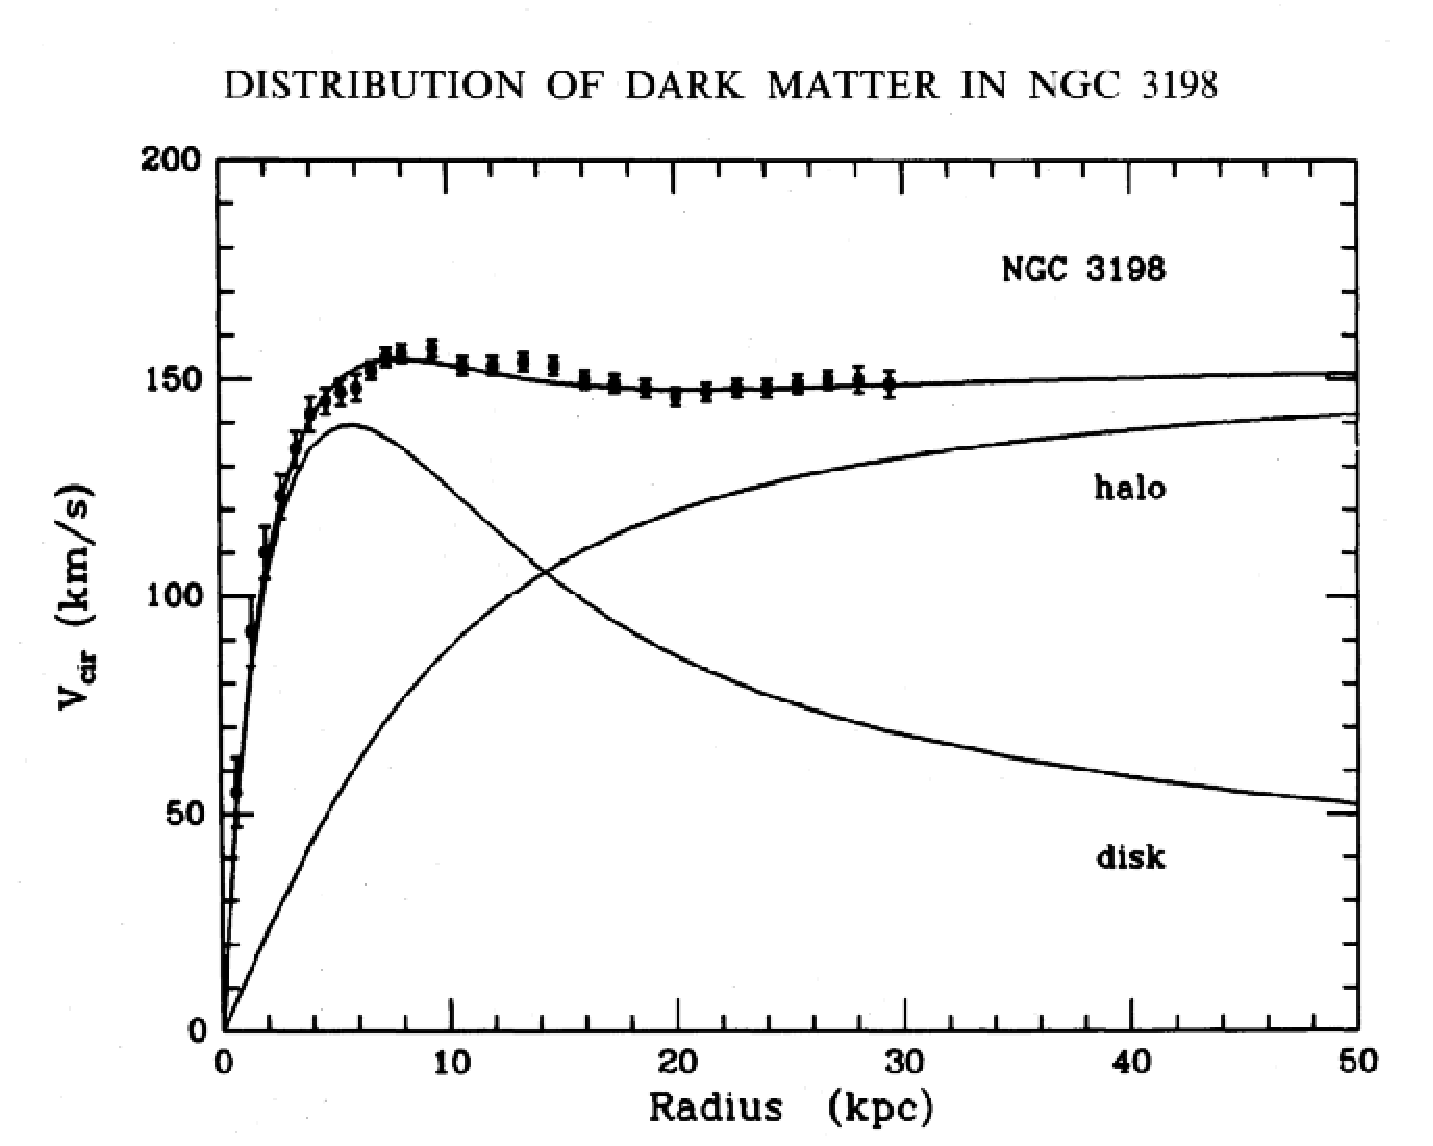
\includegraphics[width=\textwidth]{figure/Rot_vel_spir.pdf}
  \caption{Velocità di rotazione in una galassia a spirale}
  \label{vel_rot_spir}
\end{figure}
Si osserva che la velocità di rotazione galattica rimane costante fino a
distanze molto maggiori del raggio visibile $R_* \simeq 10$ kpc della galassia,
invece che diminuire con la distanza dal centro come $v_{rot}(r) \propto
r^{-1/2}$.  Questo comportamento è aspettato nell'ipotesi di esistenza della
sola materia visibile dalla 3$^a$ legge di Keplero.
\begin{figure}
  \centering{}
  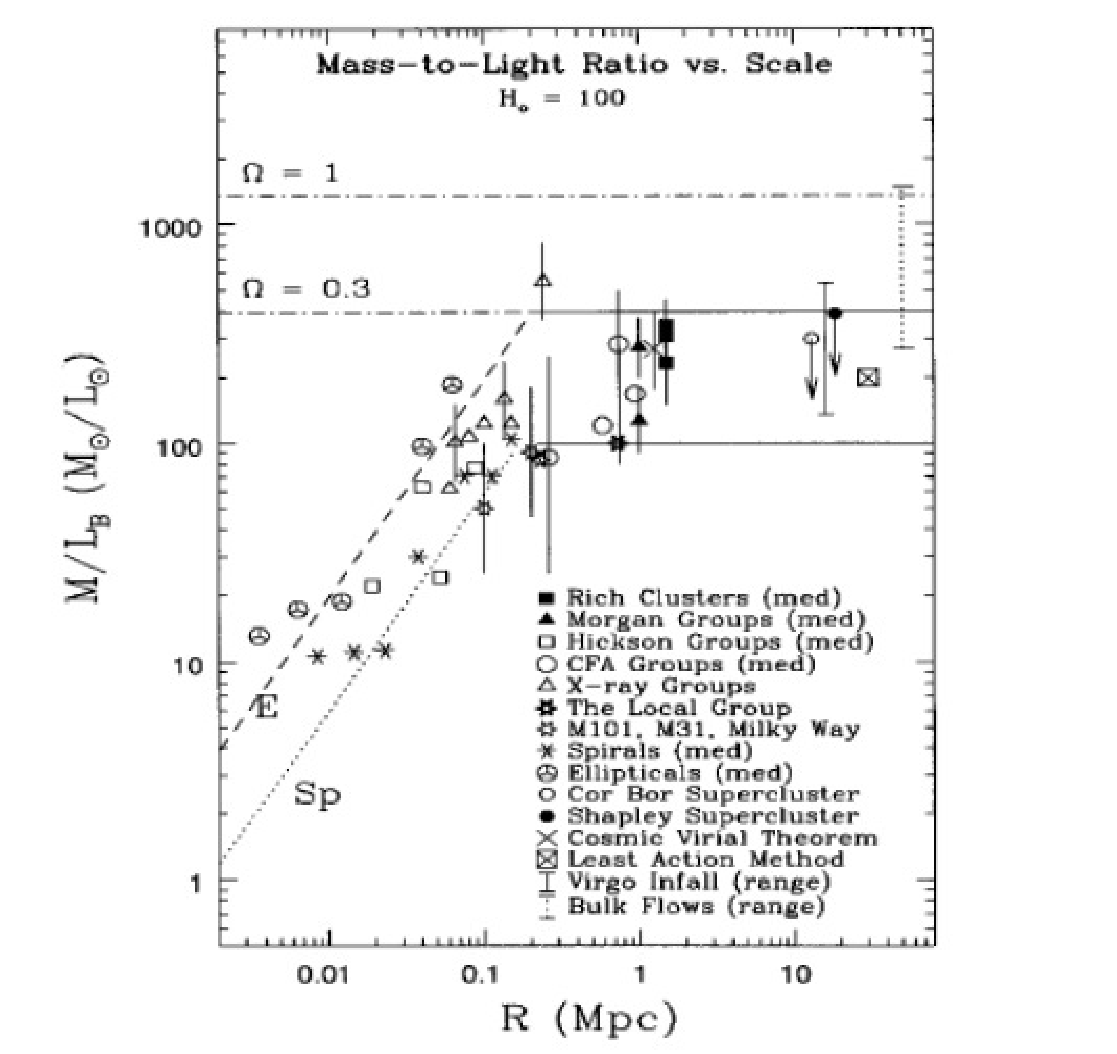
\includegraphics[width=0.7\textwidth]{figure/MoverL.pdf}
  \caption{Rapporto $M/L$ in funzione della scala}
  \label{moverl}
\end{figure}

Si deduce, quindi, che anche per le galassie a spirale $M_{din} = M_{*} +
M_{Dark}$. Se la materia oscura è distribuita con legge di densità $\rho_{Dark}
\simeq r^{-2}$ per $r>R_*$, si ha che $M_{din} \simeq r$ e quindi che
$V_{rot}(r) \propto cost$ fino a grandi distanze. Per le spirali si ottiene che
tipicamente $M_{Dark} \simeq 10 M_{*}$.

A partire dagli anni '80, osservazioni nella banda dei raggi X effettuate con
satelliti (Einstein, ROSAT, XMM, Chandra) hanno dimostrato l'esistenza di
materia oscura anche nelle galassie ellittiche (particolarmente in quelle di
grande massa) e nei clusters di galassie.  All'interno di questi sistemi
autogravitanti è presente gas diffuso (prevalentemente idrogeno ionizzato) che
si trova a temperatura $T_{gas }\simeq (0.1-1) \times 10^6$K nelle ellittiche e
$T_{gas }\simeq (3-10) \times 10^6$K nei clusters di galassie.

Il gas emette raggi X e la luminosità X totale dipende dalla massa totale di gas
$M_{gas}$ (trascurabile rispetto alla massa visibile $M_*$) e dalla temperatura
del gas $T_{gas}$.  Questa, a sua volta, attraverso il teorema del viriale e il
teorema di equipartizione dell'energia, $ m_{gas} v^2_{gas} /2 \simeq (3/2)
kT_{gas} \simeq m_{gas} G M_{din} /R$, dipende dalla massa dinamica $M_{din}$
oltre che dalle dimensioni $R$ del sistema considerato (ellittica o cluster di
galassie).  Anche in questo caso le osservazioni mostrano che $M_{din}$ è
maggiore della sola massa visibile in stelle.  Nel caso di M87, una galassia
ellittica di grande massa al centro del cluster Virgo, si trova $M_{Dark} \simeq
100 M_{*}$.
\begin{figure}
  \centering{}
  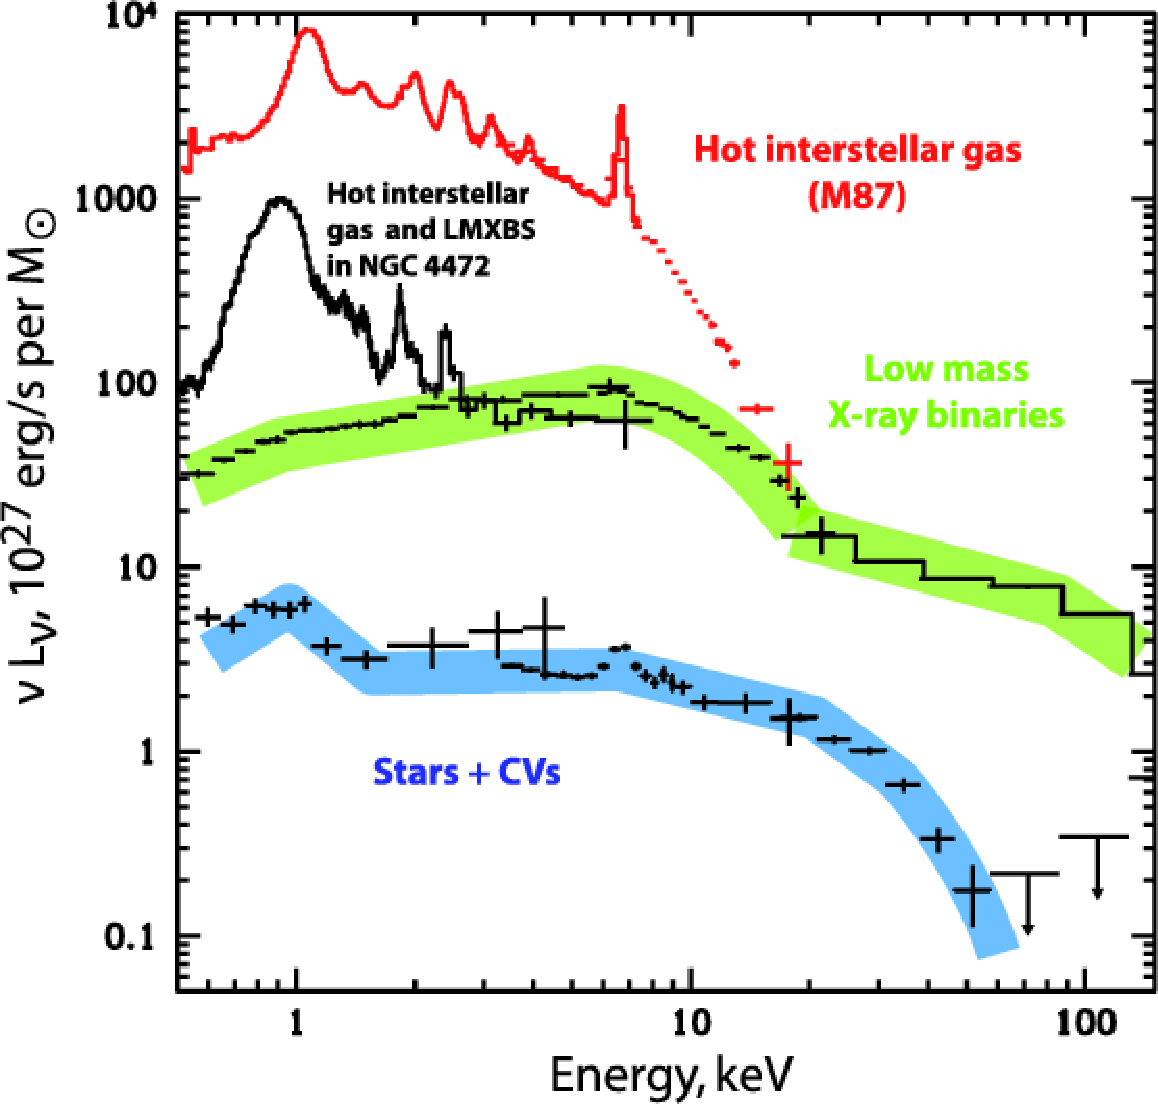
\includegraphics[width=0.7\textwidth]{figure/Xray_ellipt.pdf}
  \caption{Emissione di raggi X in alcune galassie ellittiche}
  \label{XRay_ell}
\end{figure}

\section{Principio Cosmologico}

\begin{figure}
  \centering{}
  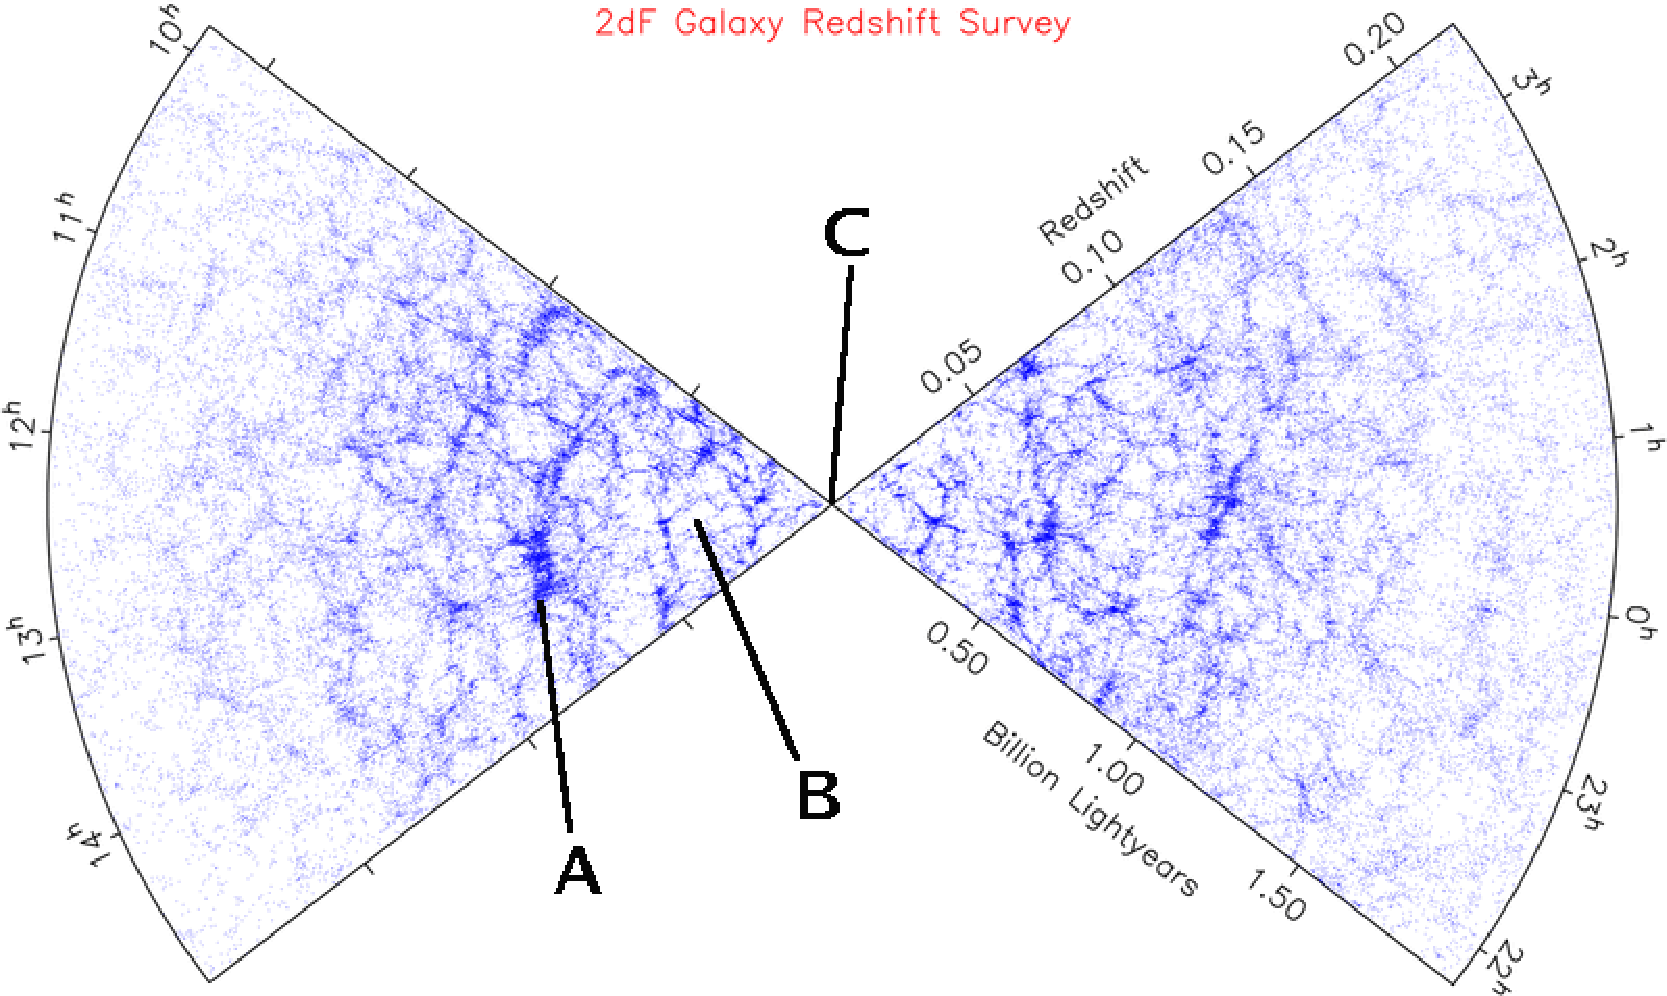
\includegraphics[width=\textwidth]{figure/2dFzcone.pdf}
  \caption{Catalogo 2dFz: distribuzione angolare di sorgenti}
  \label{cat_2d}
\end{figure}
\begin{figure}
  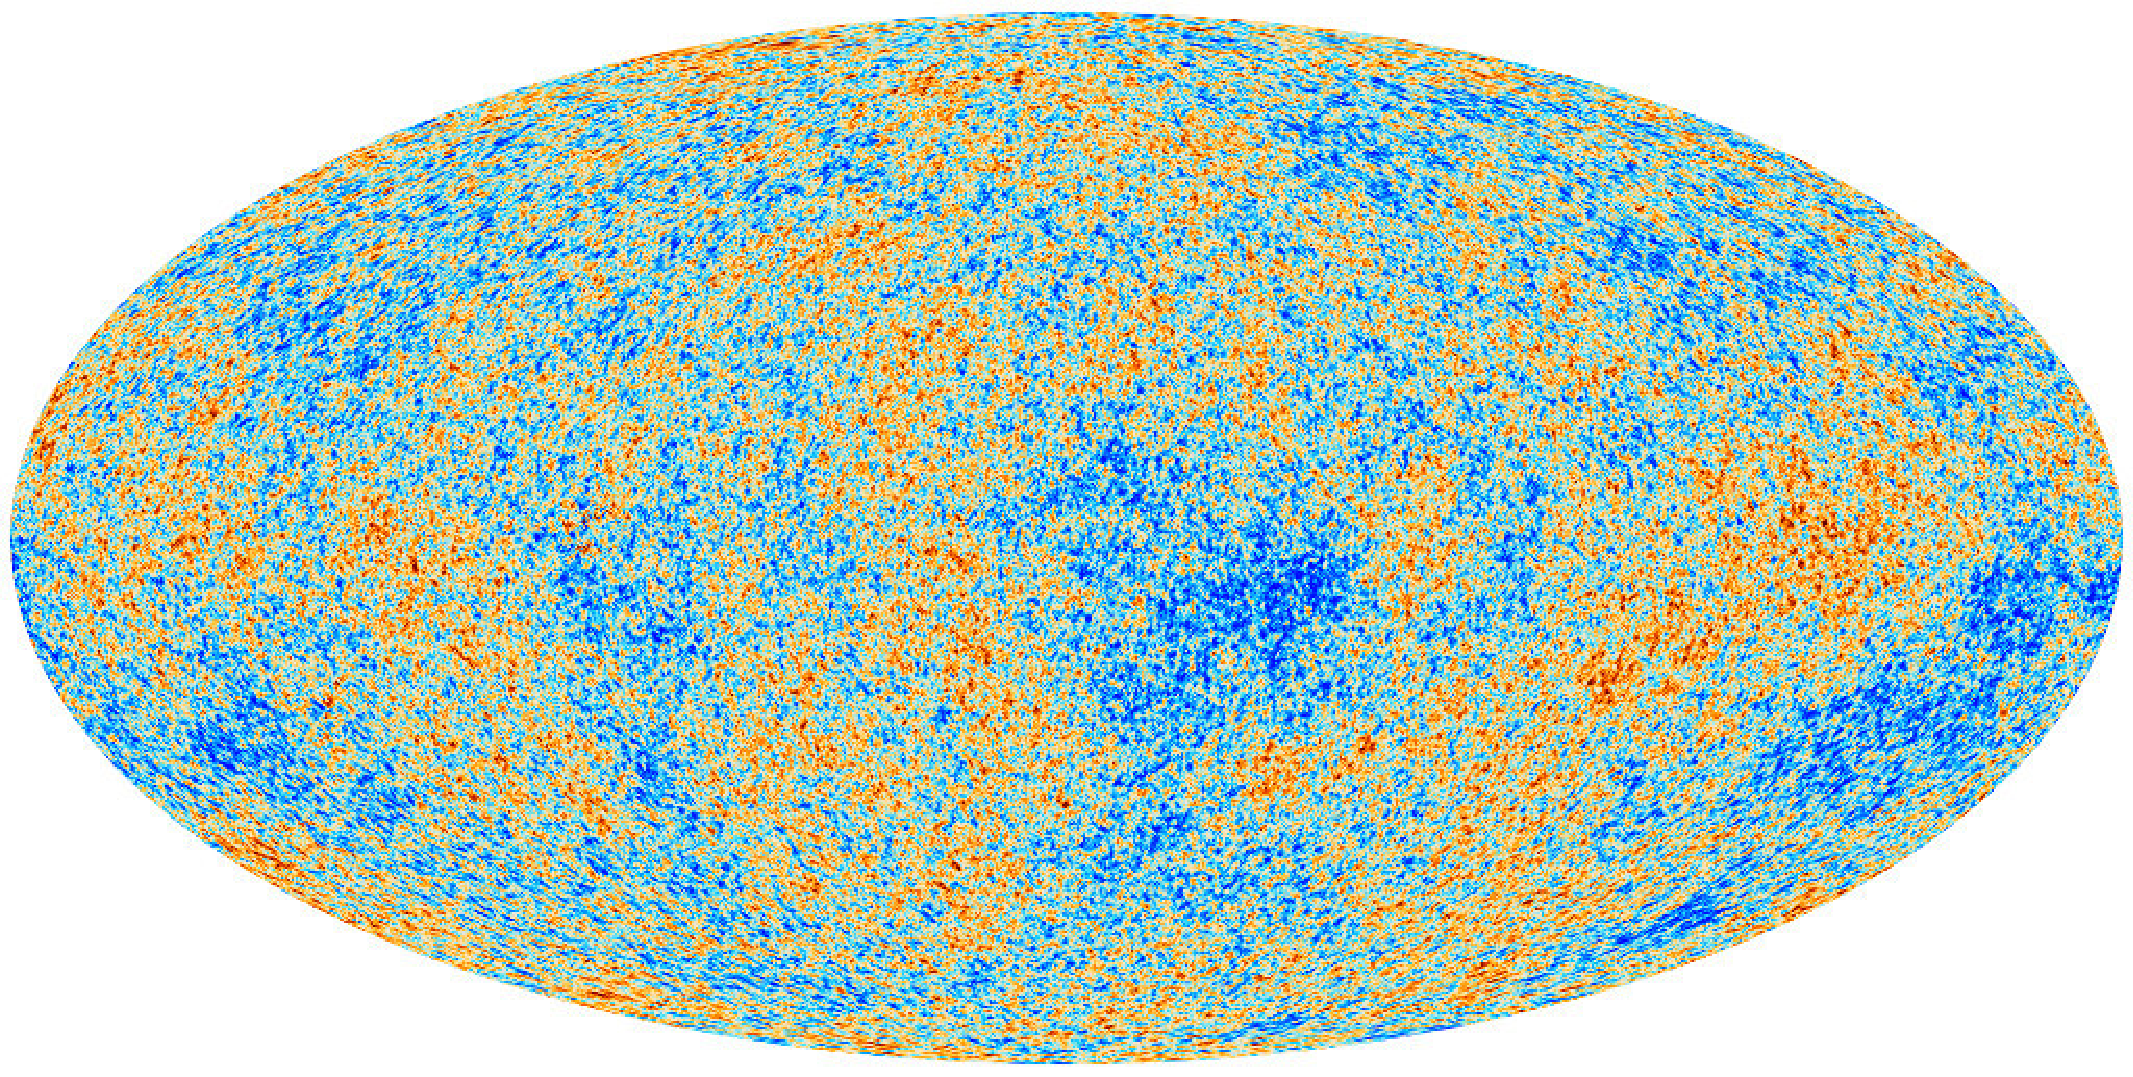
\includegraphics[width=\textwidth]{figure/Planck_CMB.pdf}
  \caption{Satellte Planck e temperatura della CMB}
  \label{sat_Planck}
\end{figure}
Il principio afferma che tutte le posizioni e tutte le direzioni direttamente
osservabili sono equivalenti: l'Universo mostra lo stesso aspetto e le stesse
proprietà fisiche in tutti i punti e in tutte le direzioni.  Le motivazioni di
carattere osservativo sono:
\begin{itemize}
\item non sono risultate anisotropie nella distribuzioni di sorgenti (nelle
  bande radio, ottico, UV, X e gamma) (vedi Fig. \ref{cat_2d}) su scala maggiore
  di 50-100 Mpc;
\item la dipendenza della velocità di recessione delle galassie con la distanza
  è la stessa in tutte le direzioni;
\item la radiazione di fondo cosmico è altamente isotropa (vedi
  Fig. \ref{sat_Planck}) poichè $\Delta T / T \simeq 10^{-5}$.
\end{itemize}

I costituenti elementari dell'Universo sono le galassie ed esiste una sequenza
di strutture (stelle, galassie, ammassi o gruppi, super-ammassi) che si arresta
sulla scala di $\simeq 100$ Mpc, oltre la quale l'Universo appare omogeneo ed
isotropo. Questa scala è molto minore della lunghezza di Hubble $R_H \simeq c
H_0$.

Comunque, non ogni oggetto può essere scelto come un buon osservatorio dal quale
verificare il Principio Cosmologico; si devono considerare solo traiettorie
fondamentali (una per ogni punto dello spazio-tempo) i cui punti possono servire
come origini di sistemi di riferimento di coordinate equivalenti: queste sono le
traiettorie di osservatori privilegiati ai quali lo spazio appare isotropo ed
omogeneo.  In prima approssimazione questi osservatori fondamentali coincidono
con le galassie in quanto ognuna di esse, a meno dei moti peculiari dovuti
all'appartenenza a sistemi autogravitanti, segue l'espansione di Hubble.

Il fatto che l'Universo presenta in ogni punto la stessa storia, fornisce una
sequenza assoluta di eventi temporali e quindi una base per definire un tempo
cosmico $t$.  Esso può essere definito come la densità o la temperatura della
CMB che variano in maniera monotona. Ad esempio per definire l'istante di
partenza di un ipotetico segnale inviato da noi verso civiltà lontane, noi
dovremmo solamente precisare che il segnale è stato inviato a $T_{CMB} =2.7$K.

\section{Geometria nell'Universo: metrica RW}

Dal punto di vista matematico il Principio Cosmologico pone restrizioni sulle
coordinate spazio-temporali ammissibili e la forma della metrica dello
spazio-tempo.

Introduciamo le coordinate spazio-temporali nel seguente modo: preliminarmente
una grandezza scalare che vari in maniera monotona (ad esempio la temperatura
del fondo cosmico nella banda delle microonde, $T_{CMB}$) fornisce un sequenza
assoluta di eventi che può essere usata per definire la scala temporale
nell'Universo.  Diremo che due eventi che accadano in posizioni differenti sono
\emph{simultanei} se una locale misura di $T_{CMB}$, effettuata al verificarsi
degli eventi, dà lo stesso valore.  L'insieme degli eventi simultanei, quindi
con stessa coordinata $t$, definisce una 3-superficie spaziale, che indichiamo
con $^{(3)}S(t)$, detta anche superficie di simultaneità.  Le coordinate
spaziali, ad esempio ($r, \theta , \phi$), sono introdotte per definire eventi
su $^{(3)}S(t)$.

Omogeneità dell'Universo significa che le condizioni fisiche sono identiche in
ogni punto di $^{(3)}S(t)$.  Quindi, queste 3-superfici devono avere curvatura
costante.

Isotropia dell'Universo significa che ad un dato tempo $t$, un osservatore
comovente con il fluido cosmologico (con le galassie) non può distinguere
direzioni spaziali attraverso misure locali.  Questo accade se e solo la
4-velocità delle galassie non ha componenti spaziali, se cioè le linee
d'Universo delle galassie sono lungo l'asse temporale.  Le galassie hanno quindi
coordinate spaziali fisse (comoventi) su $^{(3)}S$ e ciò nonostante (come
vedremo), all'aumentare di $t$, esse si allontanano l'una dall'altra a causa
dell'espansione: al crescere di $t$ la distanza tra le singole
galassie aumenta dello stesso fattore $R(t)$, mentre i rapporti di distanza
rimangono costanti.

In Cosmologia è conveniente introdurre le coordinate dello spazio-tempo in modo
che $g_{00}=-1$ e $g_{0i}=0$ (in particolare la seconda condizione permette di
sincronizzare gli orologi su di un percorso finito - vedi discussione
su~\textcite{landau:campi}).  Questo sistema è detto \emph{sincrono} e
l'espressione generale della metrica dello spazio-tempo assume la forma
\begin{equation}
  \dd\tau^2 \equiv \dd t^2 - \dd l^2 = \dd t^2 - ^{(3)}g_{ij}(t,\bm{x}) \dd x^i
  \dd x^j
\end{equation}
\begin{itemize}
\item La condizione $g_{00}=-1$ implica che per eventi che accadono nello stesso
  posto ($dx^i=0$) la differenza della coordinata temporale $dt$ misura il tempo
  proprio $d \tau$ trascorso tra i due eventi (il tempo segnato da un orologio
  che sia nello stesso posto).
\item La condizione $g_{0i}=0$ implica invece che le linee del tempo
  ($x^{\mu}(\tau)$ con $x^i=\text{cost}$) sono geodetiche dello spazio-tempo.
  Infatti poichè $g_{0i}=0$ si ha che $\tensor{\Gamma}{^{\mu}_{00}}=0$.  Con
  questo risultato (e per la condizione $dx^i=0$ per le linee del tempo),
  l'eq. della geodetica
  \begin{equation}
    \toder[2]{x^{\mu}} {\tau} + \tensor{\Gamma}{^{\mu}_{00}} \toder{x^0}{\tau}
    \toder{x^0}{\tau} = 0
  \end{equation}
  si riduce a
  \begin{equation}
    \toder[2]{x^{\mu}} {\tau} = 0
  \end{equation}
  da cui $x^{\mu}=\text{cost}$ è soluzione.
\item La stessa condizione $g_{01} =0$ implica inoltre che le linee del tempo
  sono ortogonali alle 3-superfici spaziali.  Cioè, se prendiamo un vettore
  orientato nel tempo $T^{\mu}=(1,0,0,0)$ ed uno orientato nello spazio
  $S^{\mu}=(0,S_x,S_y,S_z)$, si ha $T^{\mu} S_{\mu} = g_{0i} T^0 S^i =0$.

  Precedentemente abbiamo osservato che a causa dell'isotropia dell'Universo
  (rispetto ad osservatori fondamentali che coincidono con le galassie) la
  componente spaziale della 4-velocità delle Galassie deve essere nulla, quindi
  $V^{\mu}_G = \ltoder{x^{\mu}_G}{\tau} = (1,0,0,0)$.
\item Dalle considerazioni precedenti, segue allora che le coordinate delle
  Galassie e degli osservatori fondamentali sono fisse (labels) e che le loro
  linee d'universo sono dirette lungo l'asse del tempo risultando ortogonali
  alle 3-superfici spaziali.  Si osserva quindi che la condizione $g_{0i}=0$ è
  una condizione richiesta dall'isotropia di $^{(3)}S$.
\end{itemize}

Ora in Cosmologia, la parte spaziale della metrica $\dd
l^2=^{(3)}g_{ij}(t,\bm{x}) \dd x^i \dd x^j$ deve necessariamente avere la forma
\begin{equation}
  ^{(3)}g_{ij}(t,\bm{v}) = R^2(t) ^{3}\eta_{ij}(\bm{x})
  \label{metrica_eta}
\end{equation}
dove $^{(3)}\eta_{ij}(\bm x)$ è la metrica spaziale su una qualunque delle
3-superfici $^{(3)}S$. Infatti, il rapporto delle distanze tra due
galassie A e B
a tempi differenti non può:
\begin{itemize}
\item dipendere dalle coordinate degli estremi di A e B (omogeneità);
\item dipendere dalla direzione che connette A e B (isotropia);
\item dipendere dal modulo della distanza (per l'additività di piccole
  separazioni).
\end{itemize}
L'unica dipendenza possibile del rapporto di distanze è da una funzione del
tempo che indichiamo con $R(t)$.  Si ha allora
\begin{equation}
  \toder{l(t)}{l(t_I)} = R(t) \implies \dd l^2(t) =
  R^2(t)^{(3)}\eta_{ij}(\bm{x}) \dd x^i \dd x^j.
\end{equation}

L'isotropia attorno ad ogni punto di $^{(3)}S$ impone ulteriormente che il
termine $^{(3)}\eta_{ij}(\bm{x}) \dd x^i \dd x^j$ abbia la forma
\begin{equation}
  ^{(3)}\eta_{ij}(\bm{x}) \dd x^i \dd x^j = F(r) (\dd r^2 +r^2 \dd\Omega^2)
  \qquad\text{con}\qquad \dd\Omega^2 = \dd\theta^2 + \sin^2 \theta \dd\phi^2.
\end{equation}
Pertanto la forma completa della metrica dello spazio tempo in Cosmologia è
\begin{equation}
  \dd \tau^2 = \dd t^2 -  R^2(t) F(r) \left(\dd r^2 +r^2 \dd\Omega^2 \right)
  \label{forma_F(r)}
\end{equation}

Con il formalismo dei vettori di Killing si prova infine che la metrica deve
avere la forma stabilita da Robertson e Walker:
\begin{equation}
  d \tau^2 = dt^2 - R^2(t) \left[ \frac {dr^2}{1-kr^2} + r^2
    \left(d\theta^2+\sin^2 \theta d\phi^2\right) \right].
\end{equation}
dove $k$ è una costante che può assumere i valori $-1$, $0$, $+1$.  Questi 3
casi corrispondono a 3-superfici di curvatura costante negativa, nulla,
positiva.

\subsection{Vettori di Killing e metrica RW}

Un modo di determinare la funzione $F(r)$ in eq. \eqref{forma_F(r)} è di usare
l'omogeneità ed isotropia dello spazio, cioè la possibilità di spostare
l'origine delle coordinate in $^{(3)}S$ conservando la forma della metrica.

Consideriamo una trasformazione infinitesima di coordinate
\begin{equation}
  x^{\mu} \rightarrow x'^{\mu} = x^{\mu} + \epsilon \xi^{\mu}
  \qquad\text{con}\qquad \epsilon \ll 1
  \label{trasf_inf}
\end{equation}
che sia una isometria, cioè che lasci invariante in forma la metrica
\begin{equation}
  g'_{\mu \nu} (y) = g_{\mu \nu} (y)
  \label{inv_forma}
\end{equation}
quindi, eseguendo una trasformazione di coordinate la metrica rimane la stessa
funzione per ogni valore dell'argomento.

Vogliamo dimostrare che dalle condizioni in eq. \eqref{inv_forma} seguono le
eq. di Killing
\begin{equation}
  \xi_{\mu; \nu} + \xi_{\nu; \mu} = 0 \qquad\xi^0=0
  \label{eq_killing}
\end{equation}
La condizione $\xi^0=0$ è stata aggiunta perchè il tempo non è omogeneo.  Queste
eq. permetteranno di definire la metrica.

La dimostrazione procede nel modo seguente.  Preliminarmente, per una generica
trasformazione di coordinate $\xi^{\mu} \leftrightarrow \xi'^{\mu}$ il tensore
metrico covariante si trasforma come
\begin{equation}
  g_{\mu \nu} (x) =
  \frac{\partial x'^{\rho}  }{\partial x^{\mu}}
  \frac{\partial x'^{\sigma}}{\partial x^{\nu}}  g'_{\rho \sigma} (x')
  \label{13.1.2}
\end{equation}
Assumendo valida la condizione \eqref{inv_forma} di invarianza in forma della
metrica, possiamo sostituire nell'eq. \eqref{13.1.2} $g'_{\rho \sigma} (x')=
g_{\rho \sigma} (x')$
\begin{equation}
  g_{\mu \nu} (x) =
  \frac{\partial x'^{\rho}  }{\partial x^{\mu}}
  \frac{\partial x'^{\sigma}}{\partial x^{\nu}}  g_{\rho \sigma} (x')
\end{equation}
Si ha allora
\begin{equation}
  g_{\mu \nu} (x) =
  \left( \delta ^{\rho}_{\mu}   + \epsilon \frac{\partial \xi^{\rho}}{\partial
      x^{\mu}} \right)
  \left( \delta ^{\sigma}_{\nu} + \epsilon \frac{\partial \xi^{\sigma}}{\partial
      x^{\nu}}  \right)
  \left( g_{\rho \sigma} (x) + \frac{\partial g_{\rho \sigma}(x)}{\partial
      x^{\tau}} \epsilon \xi^{\tau} \right)
\end{equation}
e quindi al primo ordine in $\epsilon$,
\begin{equation}
  0 =  \frac{\partial \xi^{\rho}}{\partial x^{\mu}}  g_{\rho \nu} +
  \frac{\partial \xi^{\sigma}}{\partial x^{\nu}} g_{\mu \sigma} +
  \frac{\partial g_{\mu \nu}}{\partial x^{\tau}} \xi^{\tau}
  \label{eq_killing_2}
\end{equation}
che è una forma equivalente dell'eq. di Killing \eqref{eq_killing}.
Pongo ora $\xi^{\rho}   =  g^{\rho   \lambda} \xi_{\lambda}$ e
$\xi^{\sigma} =  g^{\sigma \lambda} \xi_{\lambda}$;
\begin{subequations}
  \begin{align}
    0 &= \frac{\partial ( g^{\rho   \lambda} \xi_{\lambda})  } {\partial
        x^{\mu}}  g_{\rho \nu}  +
        \frac{\partial ( g^{\sigma \lambda} \xi_{\lambda})  } {\partial x^{\nu}}
        g_{\mu \sigma} +
        \frac{\partial g_{\mu \nu}}{\partial x^{\tau}} \xi^{\tau} \\
    0 &=  \xi_{\lambda}     g_{\rho \nu}   \frac{\partial g^{\rho   \lambda}}
        {\partial x^{\mu}}  +
        g^{\rho \lambda}  g_{\rho \nu  } \frac{\partial \xi_{\lambda}     }
        {\partial x^{\mu}}  +
        \xi_{\lambda}     g_{\mu \sigma} \frac{\partial g^{\sigma \lambda} }
        {\partial x^{\nu}}  +
        g^{\sigma \lambda}g_{\mu \sigma} \frac{\partial \xi_{\lambda}      }
        {\partial x^{\nu}}   +
        \frac{\partial    g_{\mu \nu}}        {\partial x^{\tau}} \xi^{\tau}
  \end{align}
\end{subequations}
Per l'identità
\begin{equation}
  g^{\rho \lambda}g_{\rho \nu} =  \delta^{\lambda}_{\nu} \implies
  g_{\rho \nu} \frac{\partial g^{\rho _\lambda}}{\partial x^{\mu}} = -
  g^{\rho \lambda} \frac{\partial g_{\rho \nu}}{\partial x^{\mu}}
\end{equation}
abbiamo ora
\begin{equation}
 \begin{split}
   0 & = - \xi^{\rho} \frac{\partial g_{\rho \nu} } {\partial x^{\mu}} -
   \xi^{\sigma} \frac{\partial g_{\mu \sigma} } {\partial x^{\nu}} +
   \frac{\partial \xi_{\nu}} {\partial x^{\mu}} + \frac{\partial \xi_{\mu}}
   {\partial x^{\nu}} +
   \frac{\partial g_{\mu \nu}}{\partial x^{\tau}} \xi^{\tau} \\
   & = \frac{\partial \xi_{\nu}} {\partial x^{\mu}} + \frac{\partial \xi_{\mu}}
   {\partial x^{\nu}} + \xi^{\tau} \left[ \frac{\partial g_{\mu \nu} } {\partial
       x^{\tau}} - \frac{\partial g_{\tau \nu} } {\partial x^{\mu}} -
     \frac{\partial g_{\mu  \tau}} {\partial x^{\nu}} \right]\\
   & = \frac{\partial \xi_{\nu}} {\partial x^{\mu}} + \frac{\partial \xi_{\mu}}
   {\partial x^{\nu}} - 2 \xi_{\rho} \tensor{\Gamma}{^{\rho}_{\mu \nu}}
\end{split}
\end{equation}
o in maniera compatta
\begin{equation}
  0 = \xi_{\mu ; \nu} + \xi_{\nu ; \mu}.
\end{equation}
Consideriamo ora le componenti $rr$, $\theta \theta $ e $r \theta $ dell'eq. di
Killing nella forma \eqref{eq_killing_2}.  Osserviamo preliminarmente che
\begin{subequations}
  \begin{align}
    g_{\mu \nu} & = 0 \qquad\text{per}\qquad \mu \ne \nu, \\
     \parder{g_{\mu \nu}}{\phi}                  & = 0,   \\
                                         g_{r r} & = R^2(t) F(r), \\
    g_{\theta \theta}                            & = R^2(t) r^2.
  \end{align}
\end{subequations}
Per la componente $rr$ si ha:
\begin{equation}
  \frac{\partial g_{rr}}{\partial r} \xi^r +
  g_{rr}\frac{\partial \xi^r }{\partial r} +
  g_{rr}\frac{\partial \xi^r }{\partial r} =
  \frac{\partial F(r)}{\partial r} \xi^r +
  2 F(r) \frac{\partial \xi^r }{\partial r} = 0
  \label{eq_rr}
\end{equation}
Per la componente $\theta \theta$ si ha:
\begin{equation}
  \frac{\partial g_{\theta \theta}}{\partial r} \xi^r +
  g_{\theta \theta}\frac{\partial \xi^{\theta} }{\partial \theta} +
  g_{\theta \theta}\frac{\partial \xi^{\theta} }{\partial \theta} =
  \xi^r +  r \frac{\partial \xi^{\theta} }{\partial \theta} = 0
  \label{eq_thetatheta}
\end{equation}
Per la componente $r \theta$ si ha:
\begin{equation}
  \frac{\partial g_{r \theta}}{\partial r} \xi^r +
  g_{rr}\frac{\partial \xi^r       }{\partial \theta} +
  g_{\theta \theta} \frac{\partial \xi^{\theta}  }{\partial r} =
  F(r) \frac{\partial \xi^r}{\partial \theta}  +
  r^2  \frac{\partial \xi^{\theta} }{\partial r} = 0
  \label{eq_rtheta}
\end{equation}
Da eq. \eqref{eq_rr} si ha
\begin{equation}
  \frac{1}{\xi^r} \frac{\partial \xi^r}{\partial r} =-\frac{1}{2 F(r)}
  \frac{\partial F(r)}{\partial r}
\end{equation}
la cui soluzione è $\ln \xi^r =-(1/2) \ln F(r) + \text{costante}$ (rispetto a
\(r\)), cioè
\begin{equation}
  \xi^r = C(\theta, \phi) \frac{1}{\sqrt {F(r)}}
  \label{367}
\end{equation}
Da eq. \eqref{eq_thetatheta} si ha
\begin{equation}
  \frac{\partial^2 \xi^{\theta} }{\partial r \partial \theta} = -
  \frac{\partial}{\partial r } \left(\frac{\xi^r}{r}\right)
  \label{368}
\end{equation}
e da eq. \eqref{eq_rtheta}
\begin{equation}
  \frac{\partial^2 \xi^{\theta} }{\partial \theta \partial r} = -
  \frac{\partial}{\partial \theta } \left( \frac{F(r)}{r^2} \frac{\partial
      \xi^r}{\partial \theta}\right)
  \label{369}
\end{equation}
Dalle eq. \eqref{368} e \eqref{369} si ha
\begin{equation}
  F(r) \frac{\partial^2 \xi^r}{\partial \theta^2} +
  r^2 \left( \frac{\xi^r}{r^2} -\frac{1}{r} \frac{\partial \xi^r}{\partial r}
  \right) = 0
\end{equation}
e sostituendo la \eqref{367} nella precedente,  si ottiene
\begin{equation}
  \frac{1}{C} \frac{d^2 C(\theta,\phi)}{d \theta^2} =
  \frac{r^2}{\sqrt{ F(r)}} \frac{d}{dr} \left( \frac{1}{r \sqrt{F(r)}}\right)=
  \text{costante} \equiv D
\end{equation}
Dall'uguaglianza
\begin{equation}
  \frac{1}{C} \frac{d^2 C(\theta,\phi)}{d \theta^2} = D
\end{equation}
segue che necessariamente $D=-1$
\begin{equation}
  \begin{split}
    C(\theta,\phi) \propto \cos \theta & \implies
    \frac{1}{C} \frac{d^2 C(\theta,\phi)}{d \theta^2} = -1 \\
    & \implies
    \frac{r^2}{\sqrt{ F(r)}} \frac{d}{dr} \left( \frac{1}{r \sqrt{F(r)}}\right)=
    -1
  \end{split}
\end{equation}
L'eq. differenziale per $F(r)$ può essere posta nella forma
\begin{equation}
  \frac{1}{r\sqrt{F(r)}}\toder{}{r} \left(\frac{1}{r \sqrt{F(r)}}\right)= -
  \frac{1}{r^3}
\end{equation}
o, equivalentemente,
\begin{equation}
  \frac{1}{2} \dd \left( \frac{1}{r \sqrt{F(r)}} \right)^2 =
  \frac{1}{2} \dd \left(\frac{1}{r^2}\right)
\end{equation}
che si integra facilmente
\begin{equation}
  F(r) \propto \frac{1}{1+E r^2}
\end{equation}
dove $E$ è un costante.  Ridefinendo la coordinata radiale $r$ si può scrivere
infine
\begin{equation}
  F(r) \propto \frac{1}{1+k r^2}
\end{equation}
dove $k$ può assumere i valori +1, 0, -1.

\subsection{Coordinate spaziali}

Con riferimento all'eq. \eqref{metrica_eta} vogliamo ricavare la forma della
matrice $^{(3)}\eta_{ij}$.

\subsubsection{Caso $k=+1$}

L'analoga superficie in 2 dimensioni è la 2-sfera che possiamo visualizzare
nello spazio 3-dimensionale con metrica euclidea
\begin{equation}
  dl^2 = dx^2+dy^2+dz^2
\end{equation}
Appartengono alla 2-sfera i punti di coordinate $(x,y,z)$ con
\begin{equation}
  x^2+y^2+z^2=R^2
\end{equation}
con il cambiamento di variabili
\begin{equation}
  \begin{split}
    & x=R \sin \theta \cos \phi~~~~~~~~~~~~~~~~~~ 0\le \theta \le \pi \\
    & y=R \sin \theta \sin \phi~~~~~~~~~~~~~~~~~~0\le \theta \le 2 \pi \\
    & z=R \cos \theta~~~~~~~~~~~~~~~~~~~~~~~~~~~0\le \theta \le \pi
    \label{coord_sfer}
\end{split}
\end{equation}
si ha
\begin{equation}
dl^2 = R^2(d\theta^2 + \sin^2 \theta d\phi^2).
\end{equation}

In maniera analoga per la 3-sfera nello spazio euclideo 4-dimensionale si ha
\begin{subequations}
  \begin{gather}
    \dd l^2 = \dd x^2 + \dd y^2 + \dd z^2 + \dd w^2 \\
    x^2+y^2+z^2+w^2=R^2
  \end{gather}
\end{subequations}
da cui
\begin{equation}
  0 = 2 x dx + 2 y dy+ 2z dz + 2w dw \implies dw = - \frac {xdx+ydy+zdz}{\left(
      R^2-x^2-y^2-z^2 \right)^{1/2}}
\end{equation}
e quindi
\begin{equation}
dl^2 = dx^2+dy^2+dz^2 - \frac{ \left( xdx+ydy+zdz \right)^2}{\left(
    R^2-x^2-y^2-z^2 \right)}.
\end{equation}
Introduciamo le coordinate polari sferiche:
\begin{equation}
  \begin{split}
    & x=R \sin \chi \sin \theta \cos \phi                 \\
    & y=R \sin \chi \sin \theta \sin \phi~~~~~~~~~~~~~~~~~~~~~0\le \phi  \le 2 \pi \\
    & z=R \sin \chi \cos \theta~~~~~~~~~~~~~~~~~~~~~~~~~~~~~~0\le \theta \le \pi \\
    & w=R \cos \chi ~~~~~~~~~~~~~~~~~~~~~~~~~~~~~~~~~~~~~~0\le \chi \le \pi
\end{split}
\end{equation}
si ha quindi
\begin{subequations}
  \begin{align}
    x^2 + y^2 + z^2     & = R^2 \sin^2 \chi \\
    x dx + y dy + z dz  & = R^2 \sin \chi \cos \chi d \chi \\
    dx^2 + dy^2 + dz^2 & = R^2 \cos^2 \chi d \chi^2 + R^2 \sin^2 \chi d \theta^2
                         + R^2 \sin^2 \chi \sin^2 \theta d \phi^2
  \end{align}
\end{subequations}
da cui segue
\begin{equation}
  dl^2 = R^2 \left[ d \chi^2 + \sin^2 \chi \left( d \theta^2 + \sin^2 \theta d
      \phi^2 \right) \right]
\end{equation}
e posto infine $k=1$
\begin{equation}
  r= \sin \chi \implies d \chi^2 = \frac{dr^2}{1-kr^2}
\end{equation}
si ha la parte spaziale della metrica RW
\begin{equation}
  dl^2 = R^2 \left[ \frac{dr^2} {1-kr^2} + r^2 (d \theta^2+\sin^2 \theta d\phi^2) \right]
\end{equation}

Le 2-superfici a $\chi$ fissato sono 2-sfere, su cui variano $\theta$ e $\phi$,
di raggio $R \sin \chi$.  Su queste 2-sfere la distanza è $dl^2 = R^2 \sin^2
\chi (d \theta^2+\sin^2 \theta d\phi^2)$, quindi
\begin{equation}
  \sqrt{^{(2)}\eta } = R^2 \sin\chi \sin \theta \implies
  ^{(2)}V= \int_0^{\pi} \int_0^{2 \pi} R^2 \sin\chi \sin \theta d \phi d \theta =
  4\pi R^2 \sin \chi
\end{equation}
L'intero volume della 3-sfera è
\begin{equation}
  \sqrt{^{(3)}\eta } = R^3 \sin^2 \chi \sin \theta \implies
  ^{(3)}V = \int_0^{\pi} \int_0^{\pi} \int_0^{2 \pi}  R^2 \sin^2 \chi \sin \theta d
  \phi d \theta d \chi =  2 \pi^2 R^3
\end{equation}

\subsubsection{Caso $k=+0$}

È lo spazio euclideo tridimensionale descitto in coordinate polari sferiche $r=R
\chi$
\begin{equation}
  \begin{split}
    & x=R \chi \sin \theta \cos \phi~~~~~~~~~~~~~~~~~~~   0 \le \chi < \infty \\
    & y=R \chi \sin \theta \sin \phi~~~~~~~~~~~~~~~~~~~~0\le \phi  \le 2 \pi \\
    & z=R \chi \cos \theta~~~~~~~~~~~~~~~~~~~~~~~~~~~~~0\le \theta \le \pi \\
  \end{split}
\end{equation}
e distanza data da
\begin{equation}
  dl^2 = R^2 \left[ d \chi^2 + \chi^2 \left( d \theta^2+\sin^2 \theta d\phi^2
    \right) \right]
\end{equation}
L'intera 3-superficie ha volume infinito.

\subsubsection{Caso $k=-1$}

L'analoga superficie in 2-dimensioni è l'iperboloide di rivoluzione attorno
all'asse $z$ di eq.
\begin{equation}
  z^2 - (x^2+y^2) = R^2
\end{equation}
che visualizziamo immersa nel 3-spazio con metrica pseudo-euclidea
\begin{equation}
  dl^2 = dz^2-(dx^2+dy^2)
\end{equation}

Nel caso della 3-superficie con curvatura negativa abbiamo
\begin{equation}
  w^2 - (x^2+y^2+z^2) = R^2
\end{equation}
e la metrica diventa
\begin{equation}
  dl^2 = dw^2 - (dx^2+dy^2+dz^2)
\end{equation}
Le coordinate sono ora
\begin{equation}
  \begin{split}
    & x=R \sinh \chi \sin \theta \cos \phi~~~~~~~~~~~~~~~~  \\
    & y=R \sinh \chi \sin \theta \sin \phi~~~~~~~~~~~~~~~~~~~0\le \phi  \le 2 \pi \\
    & z=R \sinh \chi \cos \theta~~~~~~~~~~~~~~~~~~~~~~~~~~~~~0\le \theta \le \pi \\
    & w=R \cosh \chi ~~~~~~~~~~~~~~~~~~~~~~~~~~~~~~~~~~~~~  ~0\le \chi \le \infty    \\
  \end{split}
\end{equation}
Procedendo in modo analogo al caso $k=+1$ si ha
\begin{equation}
  dl^2 = R^2 \left[ d \chi^2 + \sinh^2 \chi \left( d \theta^2 + \sin^2 \theta d
      \phi^2 \right) \right]
\end{equation}
e posto $k=-1$
\begin{equation}
  r= \sinh \chi \implies d \chi^2 = \frac{dr^2}{1-kr^2}
\end{equation}
si ha infine
\begin{equation}
  dl^2 = R^2 \left[ \frac{dr^2} {1-kr^2} + r^2 (d \theta^2+\sin^2 \theta
    d\phi^2) \right].
\end{equation}
L'intero volume $^{(3)}V= 4 \pi R^2 \sinh^2 \chi$ è infinito.

\section{Tensore energia-impulso dell'Universo}

Come in Relatività Generale il contenuto dell'Universo (materia, radiazione,
raggi cosmici, campi magnetici, \dots) è descritto dal tensore-energia impulso
$T{\mu \nu}$.  Il Principio Cosmologico richiede che questo tensore abbia la
forma richiesta per un fluido perfetto (omogeneo ed isotropo rispetto agli
osservatori comoventi).

Dalla Relatività Speciale e il Principio di Generale Covarianza segue
\begin{equation}
  T^{\mu \nu} = ( p+ \rho) U^{\mu} U^{\nu} + p g^{\mu \nu}
\end{equation}
in cui $\rho= \rho(t)$ e $p= p(t)$ sono densità di energia e pressione totali
(proprie) misurate da osservatori comoventi.  Esse dipendono solamente dal tempo
cosmico $t$ e non dalle coordinate spaziali.

Con riferimento ai componenti dell'Universo, materia e radiazione si ha
\begin{subequations}
  \begin{align}
  \rho(t) &= \rho_m(t) + \rho_r(t), \\
  p(t) &=p_m(t)+p_r(t).
  \end{align}
\end{subequations}

Con l'uso della meccanica statistica si dimostra che
\begin{subequations}
  \begin{align}
    \rho_m &= \rho_{rm}+ u_m \\
    u_m &= \frac{p_m}{\gamma -1} \\
    \rho_{rm} &= n_m M_m c^2 \\
    p_m &\simeq n_m M_m v^2
  \end{align}
\end{subequations}
dove con $n_m$ abbiamo indicato la densità in numero di particelle, di stessa
massa $M_m$, con $u_m$ l'energia interna (termica), con $\gamma$ il rapporto di
calori specifici --- $\gamma=5/3$ (oppure $4/3$) per particelle
non-relativistiche (o relativistiche) --- e con $v$ la velocità media delle
particelle.  Nel caso di basse velocità, $v<c$, si ha $\rho_m \gg p$ e quindi si
può porre per la materia $p_m \simeq u_m \simeq 0$.

Per quanto riguarda la radiazione si ha sempre
\begin{equation}
  p_r = \frac{\rho_r}{3}
\end{equation}
e per la CMB, che ha distribuzione di corpo nero alla temperatura $T_{CMB}$,
\begin{equation}
  \rho_{CMB} = a T^4_{CMB}
\end{equation}

All'istante attuale (escludendo la Dark Energy) il maggior contributo alla
densità totale di energia nell'Universo $\rho_0$ è dato dalla materia
\begin{equation}
  \rho_0 \simeq \rho_m(0)
\end{equation}
poichè $\rho_m(0) > \rho_*(t_0) \simeq 10^{-31}$ gr cm$^{-3}$ e $\rho_r(t_0)$ è
dominata dai fotoni della CMB per i quali $\rho_{CMB}(t_0) \simeq 10^{-34}$ gr
cm$^{-3}$.

Inoltre, poiché i moti peculiari della materia (le galassie) avvengono a bassa
velocità ($\langle v_{G}\rangle \simeq 1000$ km s$^{-1}$) si può porre $p_0=0$
nell'Universo (in un modello senza DE).

In realtà indietro nel tempo l'Universo ha attraversato una fase in cui era la
radiazione a dominare.  Infatti l'applicazione della Relatività Speciale e del
Principio di Equivalenza implica che il tensore energia-impulso deve soddisfare
l'identità $\tensor{T}{^{\mu \nu}_{;\nu}}=0$ e per
$\nu=0$~\parencite[414]{weinberg:gravitation}
\begin{equation}
  R^3 \frac{dp}{dt} = \frac{d}{dt} \left[R^3 \left( \rho +p \right) \right]
\end{equation}
Questa eq. si può porre anche nella forma ($d/dt \equiv {\dot R} d/dR$)
\begin{equation}
  \frac{d}{dR} \left( \rho R^3 \right)  = -3pR^2
  \label{eq_cons}
\end{equation}
da cui è evidente che
\begin{subequations}
  \begin{align}
    \rho_m  & \simeq R^{-3} \qquad\text{se}\qquad p_m=0 \quad\text{(era
              materia)} \\
    \rho_r  & \simeq R^{-4} \qquad\text{se}\qquad p_r=\frac{\rho_r}{3}
              \quad\text{(era radiazione)}
  \end{align}
\end{subequations}

Allora ad ogni tempo cosmico abbiamo
\begin{subequations}
  \begin{align}
    \rho_m (t) &= \rho_m(t_0) \left( \frac {R(t_0)} {R(t)} \right)^3  \\
    \rho_r (t) &= \rho_r(t_0) \left( \frac {R(t_0)} {R(t)} \right)^4
  \end{align}
\end{subequations}
L'ultima relazione, poiché per la radiazione di fondo cosmico $\rho_r \propto
T^4_{CMB}$, implica che $T_{CMB}(t)$ cambia nel tempo secondo la relazione
\begin{equation}
  T_{CMB}(t) = T_{CMB}(t_0) \left( \frac {R(t_0)} {R(t)} \right).
\end{equation}
Quindi l'Universo oggi è dominato dalla materia, ma poichè indietro nel tempo
$\rho_r(t)$ cresce più velocemente di $\rho_m(t)$, esisterà nel passato un'era
della radiazione in cui $\rho(t) \simeq \rho_r(t)$.

Con riferimento all'epoca in cui le galassie sono già formate, possiamo definire
una densità di corrente di galassie
\begin{equation}
  J^{\mu}_{~G}(t) = n_G(t) U^{\mu}
  \label{154}
\end{equation}
dove $n_G(t)$ è la densità propria di galassie e $U^{\mu}=(1,0,0,0)$ è la
4-velocità delle galassie.  La conservazione del numero di galassie sarà
espressa dalla relazione
\begin{equation}
  J^{\mu}_{G~~;\mu} \equiv \frac{1}{\sqrt{g}} \frac{\partial}{\partial t}
  (\sqrt{g} n_G)
\end{equation}
Il determinante della metrica RW (cambiato di segno) è
\begin{equation}
  g=R^6(t) r^4 (1-kr^2)^{-1} \sin \theta ^2
\end{equation}
e quindi l'eq. \eqref{154} diventa
\begin{equation}
  n_G(t) R^3(t) = \text{costante}.
\end{equation}
Nota che $n_G(t)$ è la densità in numero di galassie per unità di volume
proprio\footnote{L'osservatore comovente usa una misura di lunghezza $l$ che non
  varia con l'espansione dell'Universo, conta il numero totale $N_G$ di galassie
  entro un volume proprio di dimensioni $l^3$ e calcola $n_G = N_G/l^3$.}  ed
esso diminuisce (aumenta) a seconda che l'Universo si espande (si contrae).
Allo stesso tempo $n_G(t) R^3(t)$ è la densità di galassie per unità di volume
comovente, che rimane costante nel tempo.

Allora la dipendenza da $R(t)$ delle densità $\rho_m(t)$ e $\rho_r(t)$ ha una
semplice interpretazione.  Se l'Universo è in espansione, la densità propria di
oggetti (galassie o fotoni) diminuisce come $R^{-3}$.  Per la materia non
relativistica, la cui densità di energia è dominata dalla massa a riposo, si ha
$\rho_m (t) \simeq n_G (t) M_m c^2 \simeq R^{-3}$.  Per quanto riguarda la
radiazione, il numero proprio di fotoni $n_{\gamma} \simeq R^{-3}$, ma la
densità di energia $\rho_r \simeq n_{\gamma} E_{\gamma}$ varia come $\simeq
R^{-4}$, poichè l'energia di ciascun fotone $E_{\gamma} = hc/\lambda$ scala come
$\simeq R^{-1}$.

\section{Distanza propria}

La distanza tra due galassie, ad esempio la nostra Galassia ad $r=0$ ed una
galassia esterna con coordinata radiale $r_1$, si calcola ad ogni tempo dalla
metrica RW ponendo $dt=0$, il che esprime la condizione di contemporameità, e $d
\theta = d \phi =0$, come è sempre possibile fare con una opportuna orientazione
del sistema di coordinate.  In questo modo si ottiene
\begin{equation}
  D_P(t) = R(t) \int_0^{r_1} \frac{dr}{\sqrt{1-kr^2}} \equiv R(t) f(r_1)
  \label{dprop}
\end{equation}
dove $f(r_1)$ è data da
\begin{equation}
  f(r_{1}) =
  \begin{cases}
    \arcsin r_{1}  & \text{se } k = 1, \\
    r_{1}        & \text{se } k = 0, \\
    \arcsinh r_{1} & \text{se } k = -1.
  \end{cases}
\end{equation}
Per piccoli valori di $r_1\ll 1$ si ha
\begin{subequations}
  \begin{align}
    \arcsin r_1 &= r_1 +\frac{r_1^3}{6}  \simeq r_1 \\
    \arcsinh r_1 &= r_1 -\frac{r_1^3}{6}  \simeq r_1
  \end{align}
\end{subequations}
e la distanza propria diventa:
\begin{equation}
  D_P(t) = R(t) r_1 + O(r_1^3) \qquad\text{se}\qquad r_1 \ll 1.
\end{equation}

Dal punto di vista osservativo la distanza propria $D_P(t)$ non ha significato
fisico perchè le misure di distanza eseguibili non possono avvenire a uguale
tempo cosmico $t$.  La misura di distanze in Cosmologia presuppone la
propagazione di segnali elettromagnetici che sono emessi al tempo $t_1$ da una
galassia esterna (nella posizione $r_1$) e che si propagano fino a noi (in
$r=0$) che li riceviamo all'istante $t_0>t_1$.

Si definisce \emph{red-shift cosmologico} la quantità
\begin{equation}
  z = 1 + \frac{R(t_0)}{R(t)}.
\end{equation}
Si stabilisce così una corrispondenza biunivoca tra tempo $t$ e red-shift $z$:
l'istante attuale $t_0$ corrisponde a $z=0$; indietro nel tempo $R(t)$ decresce
così che $z$ cresce, e per $t \to 0$ si ha $z \to +\infty$.  Gli oggetti più
lontani (e più vecchi) che noi oggi osserviamo sono i QSOs che si trovano $z
\simeq 5$.  Il tempo corrispondente a tale valore di $z$ risulta una frazione
apprezzabile dell'età dell'Universo.

Derivando rispetto al tempo la relazione \eqref{dprop} e prendendo il risultato
al tempo attuale, si trova in modo formale la legge di Hubble
\begin{equation}
  V_H = \frac {dD_P(t)}{dt}|_{t=t_0} = \dot{R}_0 f(r_1) = H_0 D
\end{equation}
dove si è definita la costante di Hubble
\begin{equation}
  H_0=\frac{\dot{R}_0}{R_0}.
\end{equation}

\section{Red-shift cosmologico}

Consideriamo un segnale elettromagnetico emesso al tempo $t=t_1$ da una galassia
lontana, con coordinata radiale $r=r_1$.  Il segnale è da noi ricevuto in $r=0$
al tempo $t_0>t_1$.  Dal Principio di Equivalenza la velocità di propagazione è
pari a $c$, e quindi $d \tau= 0$.  Se orientiamo gli assi in modo che $d \theta
= d \phi=0$, dalla metrica RW si ha
\begin{equation}
  dt = R(t) \frac{dr}{\sqrt{1-kr^2}}
\end{equation}
e integrando (osserva che $dr<0$)
\begin{equation}
  \int_{t_1}^{t_0} \frac{dt}{R(t)} = \int_0^{r_1} \frac{dr}{\sqrt{1-kr^2}}
  \equiv f(r_1)
\end{equation}
Si stabilisce quindi una corrispondenza implicita tra $r_1$, $t_1$, $t_0$.

Consideriamo ora una sola lunghezza d'onda: la prima cresta d'onda parte al
tempo $t_1$ e arriva al tempo $t_0$ dato da
\begin{equation}
  \int_{t_1}^{t_0} \frac{dt}{R(t)} =  f(r_1).
\end{equation}
La cresta successiva parte al tempo $t_1+\Delta t_1$ e arriva al tempo $t_0+
\Delta t_0$ dato ancora da
\begin{equation}
  \int_{t_1+ \Delta t_1}^{t_0+ \Delta t_0} \frac{dt}{R(t)} =  f(r_1).
\end{equation}
Da queste due relazioni si ricava l'uguaglianza
\begin{equation}
  \int_{t_1}^{t_0} \frac{dt}{R(t)} =  \int_{t_1+ \Delta t_1}^{t_0+ \Delta t_0}
  \frac{dt}{R(t)}
\end{equation}
che implica
\begin{equation}
  \int_{t_1}^{t_1+\Delta t_1} \frac{dt}{R(t)} =  \int_{t_0}^{t_0+ \Delta t_0}
  \frac{dt}{R(t)}
  \label{169}
\end{equation}

Ora i tempi $\Delta t_1= 1/\nu_1$ e $\Delta t_0 = 1/\nu_0$ corrispondono a
periodi del segnale elettromagnetico in partenza e in arrivo che, anche
considerando le onde di lunghezza d'onda massima che arrivano a terra (nel radio
$\Delta t \simeq 10^{-7}$ sec), sono estremamente più piccoli dei tempi su cui
varia $R$.  Perciò possiamo approssimare l'eq. \eqref{169} con
\begin{equation}
  \frac{\Delta t_1}{R_1} = \frac{\Delta t_0}{R_0}
\end{equation}
o, equivalentemente,
\begin{equation}
  \frac{\nu_0}{\nu_1} = \frac{\lambda_1}{\lambda_0}= \frac{R(t_1)}{R(t_0)}
  \implies \lambda \sim R(t).
\end{equation}
per cui la lunghezza d'onda della radiazione di fondo cosmico scala come $R$. In
termini del red-shift $z$ si ha
\begin{equation}
1+z \equiv \frac {R(t_0)} {R(t_1)} = \frac{\lambda_0} {\lambda_1}
\end{equation}
Le misure di red-shift cosmologico mostrano che $z>0$ e pertanto che l'Universo
oggi è in espansione.

Il red-shift è un effetto di scala e la sua legge generale è $\lambda \sim R$.
Comunque, per oggetti vicini esso si riduce all'effetto Doppler.  Infatti,
ponendo $\Delta t = t_0-t_1 >0 $, in prima approssimazione si ha
\begin{equation}
  1+z = \frac{R_0} {R(t_0-\Delta t)} \simeq \frac{R_0} {R_0 -\dot{R}_0 \Delta t}
  \simeq 1 + \frac {\dot{R}_0} {R_0} \Delta t
\end{equation}
da cui
\begin{equation}
  z \simeq \frac {\dot{R}_0} {R_0} \Delta t
  \label{137}
\end{equation}
Nella stessa approssimazione si ha
\begin{equation}
  \int_{t_0-\Delta t}^{t_0} \frac{dt}{R(t)} \simeq \frac{\Delta t}{R_0}
\end{equation}
mentre
\begin{equation}
  \int_{t_0-\Delta t}^{t_0} \frac{dt}{R(t)} = f(r_1) \simeq r_1
\end{equation}
Dunque $\Delta t =  R_0 r_1$ e sostituendo nella \eqref{137}
\begin{equation}
  z \simeq \frac{\dot{R_0}}{c} r_1 \simeq \frac {v_H}{c}
\end{equation}
che è la forma in cui si pone l'effetto Doppler.  Si ha anche:
\begin{equation}
  v_H \simeq {\dot{R_0}} r_1 = \frac {\dot{R_0} R_0  r_1} {R_0} = {H_0}{D}
\end{equation}
e dunque ancora la legge di Hubble.  Notiamo infine che la legge di Hubble
stabilisce una corrispondenza tra $z$ e $D$
\begin{equation}
  D = \frac{c}{H_0} z = z ~ 4000 ~ {\rm Mpc}  ~
 \left( \frac { 75 ~{\rm km/(s ~ Mpc) }} {H_0} \right)
\end{equation}

\section{Relazione tra red-shift e distanza di luminosità}

In geometria euclidea si definisce la distanza di luminosità $d_L$ a partire
dalla relazione tra flusso osservato $F$ e luminosità assoluta $L$
\begin{equation}
  F = \frac{L}{4 \pi d^2_L} \iff d_L = \left(\frac{L}{4 \pi F} \right)^{1/2}.
  \label{dist_eucl}
\end{equation}
Qui la quantità $4 \pi d^2_L \equiv A$ è l'area della sfera di raggio $d_L$.  In
Cosmologia l'area della sfera comovente di raggio $d_L$, centrata sulla sorgente
che si trova a distanza $r_1$, è calcolata al tempo $t_0$ dalla metrica RW
ponendo $r=r_1$, $t=t_0$ ($dr=0$ e $dt=0$)
\begin{equation}
  A = \int_0^{2 \pi} \int_{0}^{\pi} \sqrt {^{(2)}g} d\theta d\phi = R^2(t_0)
  r^2_1 \int_0^{2 \pi} \int_{0}^{\pi} \sin \theta d\theta d\phi = 4 \pi R^2_0
  r^2_1.
\end{equation}
Quindi per un osservatore fisso in un punto generico della sfera comovente,
nell'ipotesi di propagazione istantanea, il flusso ricevuto sarebbe dato da
\begin{equation}
  F = \frac{L}{4 \pi R^2_0 r^2_1}
\end{equation}
Ora, però, dobbiamo tenere conto dell'espansione dell'Universo per cui:
\begin{itemize}
\item i fotoni arrivano con frequenza minore: $h \nu \to h \nu /(1+z)$;
\item la "distanza temporale" tra i singoli fotoni viene aumentata
  dall'espansione, ovvero il ritmo di arrivo dei fotoni è rallentato rispetto a
  quello di emissione del fattore $1/(1+z)$.  Quindi
  \begin{equation}
    F = \frac{L}{4 \pi R^2_0 r^2_1} \frac{1}{(1+z)^2} = \frac{L}{4 \pi R^2_0
      r^2_1} \frac{R^2_1}{R^2_0} = \frac{L R^2_1}{4 \pi R^4_0 r^2_1}.
  \end{equation}
  Dalla relazione \eqref{dist_eucl} a questo flusso $F$ corrisponde la distanza
  \begin{equation}
    d_L = \frac{R^2_0 r_1} {R_1} \equiv R_0 r_1 (1+z)
    \label{dis_lum}
  \end{equation}
\end{itemize}

{\bf Vogliamo ora ricavare una relazione $d_L=d_L(z)$ tra red-shift e distanza di
luminosità, che sia indipendente da un particolare modello cosmologico}. Tale
relazione, come vedremo, introdurrà due parametri che risultano rilevanti in
Cosmologia. Pertanto un programma osservativo con misure (fotometriche) di
distanza e (spettroscopiche) di red-shift di una stessa classe di oggetti
(candele standard) con luminosità $L$ costante, permetterebbe di determinare i
valori dei parametri cosmologici introdotti.

Consideriamo una classe di indicatori di distanza di stessa luminosità assoluta
$L$. Partiamo dalla relazione \eqref{dis_lum} operando espansioni al 2$^0$
ordine in $z$, $(t_1-t_0)$, $r_1$.  Sia $\Delta t= t_1-t_0 <0$; si ha
\begin{equation}
  R(t_1) \simeq R(t_0) \left( 1+H_0 \Delta t -\frac{1}{2} H^2_0 q_0 \Delta
    t^2+\cdots \right)
\end{equation}
Qui $H_0$ è la costante di Hubble e $q_0$ è il parametro di decelerazione
\begin{subequations}
  \begin{align}
    H_0 &= \frac{{\dot R}_0 }{R_0}, \\
    q_0 &= - {\ddot R}_0 \frac{R_0}{{\dot R}^2_0}.
  \end{align}
\end{subequations}
Abbiamo quindi
\begin{equation}
  \begin{split}
    1+z \equiv \frac{R_0}{R_1} & \simeq \frac{R_0}{R_0 \left[ 1+H_0 \Delta t -
        \frac{1}{2} q_0 H^2_0 \Delta t^2+\cdots\right]} \\
    & \simeq  1- H_0 \Delta t +\frac{1}{2} q_0 H^2_0 \Delta t^2 + H^2_0 \Delta
    t^2+\cdots
  \end{split}
\end{equation}
quindi
\begin{equation}
  z \simeq - H_0 \Delta t +\left( 1+\frac{1}{2} q_0 \right) H^2_0 \Delta t^2
  +\cdots
\end{equation}
da cui, per inversione della serie di potenze, si ricava
\begin{equation}
  -\Delta t \simeq  \frac{1}{H_0} \left[ z - \left( 1 +\frac{1}{2} q_0 \right)
    z^2 +\cdots \right]
\end{equation}
Consideriamo ora la relazione ottenuta dalla metrica RW ponendo $d\tau=0$
\begin{equation}
  \int_0^{r_1} \frac{dr}{\sqrt{1-kr^2}} = \int_{t_1}^{t_0} \frac{dt}{R(t)}
\end{equation}
Il primo termine è $ \simeq r_1 + O(r^3_1)$; il secondo termine è
\begin{equation}
  \int_{\Delta t}^{0} \frac{d(\Delta t')}{R_0} \left[ 1-H_0 \Delta t' + \left(1+
      \frac{1}{2} q_0 \right) H^2_0
    \Delta t' +\cdots \right] \simeq \frac{1}{R_0} \left[ -\Delta t +
    \frac{1}{2} H_0 \Delta t^2+\cdots \right]
\end{equation}
Complessivamente si ha:
\begin{equation}
  \begin{split}
    r_1 & \simeq \frac{1}{R_0} \left[ -\Delta t + \frac{1}{2}H_0 \Delta t^2 + \cdots \right] \\
    & \simeq \frac{1}{R_0} \left[
      \frac{z}{H_0} -
      \frac{1}{H_0} \left(1 + \frac{1}{2} q_0 \right) z^2
      + \frac{H_0}{2} \frac{z^2}{H^2_0} + \cdots \right]
  \end{split}
\end{equation}
da cui si ottiene
\begin{equation}
  r(z) \simeq \frac{z}{R_0 H_0} \left[ 1- \left( \frac{1+q_0}{2}\right) z +
    \cdots \right]
\end{equation}
La distanza di luminosità è allora data da
\begin{equation}
  d_L \equiv R_0 r_1 (1+z)
  \simeq R_0 \frac{z}{R_0 H_0} \left[ 1 - \left( \frac{1+q_0}{2} \right) z +
    \cdots \right] (1+z)
\end{equation}
ed infine
\begin{equation}
  d_L = \frac{cz}{H_0} \left[ 1 + \left( \frac{1-q_0}{2} \right) z + \cdots \right]
  \label{1468}
\end{equation}
{bf Tale relazione è indipendente dal modello cosmologico utilizzato}. All'ordine più
basso riprendiamo la legge di Hubble.

Possiamo esprimere il flusso osservato in termini di $z$.  Si ottiene
\begin{equation}
  F \equiv \frac{L}{4 \pi d^2_L} \simeq \frac{L H^2_0}{4 \pi c^2}
  \left[ \frac {1+\left (q_0-1 \right) z}{z^2} \right]
  \label{160}
\end{equation}
Passando dal flusso $F$ alle magnitudini apparenti $m$ si ha
\begin{equation}
  F = 2.52 \times 10^{-5} \times 10^{-\frac{2}{5} m} \iff
  m = -2.5 \log \frac {F}{2.52 \times 10^{-5}}
\end{equation}
e definendo la magnitudine assoluta $M$ come la magnitudine apparente
che la sorgente avrebbe se posta a 10 pc
\begin{equation}
  L = 3.02 \times 10^{35} \times 10^{-\frac{2}{5} M}.
\end{equation}
La relazione tra $M$ ed $m$ è
\begin{equation}
  M = m +2.5 \log \left( \frac{D(pc)}{10 pc}\right)^{-2}.
\end{equation}

La relazione tra flusso, luminosità assoluta e red-shift in eq. \eqref{160},
diventa ora
\begin{equation}
  m-M = 25 - 5 \log H_0 {\rm(km/s/Mpc)}+ 5 \log cz {\rm (km/sec)}+ 1.086 (1-q_0)
  z
\end{equation}
o, equivalentemente,
\begin{equation}
  \log (cz) = \frac{m}{z} - 0.217 (1-q_0)z +\log H_0 - \frac{M}{5} -5.
\end{equation}

Le quantità misurabili sono $m$ e $z$ e con queste si può costruire un diagramma
osservativo $m-z$ noto come \emph{diagramma di Hubble}.  Nel caso di misure
locali ($z \to 0$) il termine $(1-q_0)z$ si può trascurare; $z$ deve comunque
essere sufficientemente grande da corrispondere a velocità di espansione ($v_H
\simeq zc$) maggiori delle velocità peculiari delle galassie ($\simeq 1000$
km/s).  In questo modo si determina $H_0 \simeq 65 \pm 3$ km/s/Mpc.

Le difficoltà nascono quando si vuole determinare $q_0$, in quanto bisogna usare
come indicatori di distanza galassie lontane ($z \simeq 1$) la cui luminosità
(che deve anche essere grande) è soggetta a forti effetti evolutivi.  Fino agli
anni '90 il programma di Hubble non è stato portato a termine in quanto dai
diagrammi $m-z$ si determina $q_0 = 0.5 \pm 0.5$, quindi con un grande errore.

Verso la fine degli anni '90 il programma è stato ripreso da Perlmutter e Riess
usando come indicatori di distanza Supernovae (di tipo Ia) piuttosto che
galassie.

\section{Relazione di Mattig: $d_L(z)$ per i modelli di Friedmann. }

Cerchiamo una relazione esatta tra coordinata comovente $r_1$ e red-shift $z$ per
il caso in cui $R(t)$ .
Consideriamo un segnale emesso al tempo $t_1$ da una galassia in $r=r_1$ e che
ci raggiunge in $r=0$ all'istante attuale $t_0$. Integrando radialmente la
metrica di RW, si ha
\begin{equation}
  \int_0^{r_1} \frac{dr}{\sqrt{1-kr^2}} = \int_{t_1}^{t_0} \frac{dt}{R(t)} =
  \int_{R_1}^{R_0} \frac{dR}{R \dot{R}}
\end{equation}
Utilizzando l'eq. di Friedmann \eqref{eq:friedmann} (nella forma \eqref{2.40}),
con $x=R(t)/R_0$ possiamo scrivere l'integrale sopra come
\begin{equation}
  \int_0^{r_1} \frac{dr}{\sqrt{1-kr^2}} = \frac{1}{R_0 H_0}
  \int_{(1+z)^{-1}}^{1} \left(1-2q_0+ \frac{2q_0}{x} \right)^{-1/2} \frac{dx}{x}
\end{equation}
Supponiamo ora di essere nel caso $k=1 \implies q_0>1/2$.  Operiamo la trasformazione
\begin{equation}
  \begin{split}
    & x= \frac{2q_0}{2q_0-1} \sin^2 \theta ~~~\rightarrow~~~ dx = \frac{2q_0}{2q_0-1} 2 \sin \theta \cos \theta \\
    & x=1 ~~~\rightarrow~~~ \frac{2q_0}{2q_0-1} \sin^2 \theta_0 =1 ~~~\rightarrow~~~
    \theta_0= \arcsin \left(\frac{2q_0-1}{2q_0}\right)^{1/2} \\
    & x= \frac{1}{1+z} ~~~\rightarrow~~~ \frac{2q_0}{2q_0-1} \sin^2 \theta= \frac{1}{1+z} ~~~\rightarrow~~~
    \theta = \arcsin \left(\frac{2q_0-1}{2q_0(1+z)}\right)^{1/2} \\
  \end{split}
  \label{posizioni_mattig}
\end{equation}
si ha allora
\begin{equation}
  \begin{split}
    \arcsin r_1 & = \frac{1}{R_0 H_0} \int_{\theta}^{\theta_0}
    \frac{ \left(\frac {2q_0}{2q_0-1}\right)  2 \sin \theta \cos \theta d\theta}
    { \left(\frac{2q_0}{2q_0-1}\right) \sin^2 \theta
      \left( 1-2q_0 + 2q_0 \frac{(2q_0-1)}{ 2q_0 \sin^2 \theta} \right)^{1/2}} \\
    & = \frac{2}{R_0 H_0 \sqrt{2q_0-1}}  \int_{\theta}^{\theta_0}
    \frac{\cos \theta d \theta}{\sin \theta \left(\frac{1}{\sin^2 \theta} -1 \right)^{1/2}} \\
    & = \frac{2}{R_0 H_0 \sqrt{2q_0-1}}  \int_{\theta}^{\theta_0} d \theta \\
    & = \frac{2}{R_0 H_0 \sqrt{2q_0-1}}
    \left[ \arcsin \left(\frac{2q_0-1}{2q_0}\right)^{1/2} -
      \arcsin \left(\frac{2q_0-1}{2q_0(1+z)}\right)^{1/2}  \right]
  \end{split}
\end{equation}
Prendendo il $\sin$ di questa equazione ed usando la relazione $\sin(a-b)= \sin
a \cos b - \ sin b \cos a$ si ha infine la relazione di Mattig
\begin{equation}
  r_1 = \frac{z q_0 +(q_0-1) (-1+\sqrt{2q_0z+1})}{R_0 H_0 q^2_0 (1+z)}
  \label{mattig}
\end{equation}
Questa è un'espressione generale di $r_1=r_1(z)$ valida per i modelli di
Friedmann e per qualunque valore di $q_0$.  Il caso $k=-1$ si ottiene in modo
analogo ponendo $\sinh $ al posto di $\sin$ in eq. \eqref{posizioni_mattig}.  La
distanza di luminosità diventa
\begin{equation}
  d_L \equiv R_0 r_1 (1+z) = \frac{1}{H_0 q^2_0} \left[ z q_0 +(q_0-1)
    (-1+\sqrt{2q_0z+1}) \right].
\label{15324}
\end{equation}
Questa è la formula esatta per i modelli di Friedmann da comparare con la
formula approssimata \eqref{1468}
\begin{equation}
  d_l \simeq \frac{1}{H_0} [z + \frac{1}{2} (1-q_0) z^2] + O(z^3)
\end{equation}
La differenza tra le due formule è zero per $q_0=0$ e $q_0=1$ è minore del 10\%
per $0<z<1.5$~\parencite{weinberg:gravitation}.  Quindi nella determinazione di
$q_0$ attraverso il diagramma di Hubble non vi è una sostanziale differenza tra
la formula esatta e la formula approssimata, almeno fino a che $z$ non è troppo
grande.

\section{Distanza di diametro angolare}

Supponiamo di conoscere la lunghezza propria $D$ di un oggetto (una galassia)
alla distanza radiale $r_1$, disposto per semplicità perpendicolarmente alla
linea di vista.  Misurandone la dimensione angolare $\Delta \theta$ possiamo
definire una \emph{distanza di diametro angolare} $d_A$ per mezzo della
relazione
\begin{equation}
  d_A = \frac{D}{\Delta \theta}
\end{equation}
\begin{figure}
  \centering{}
  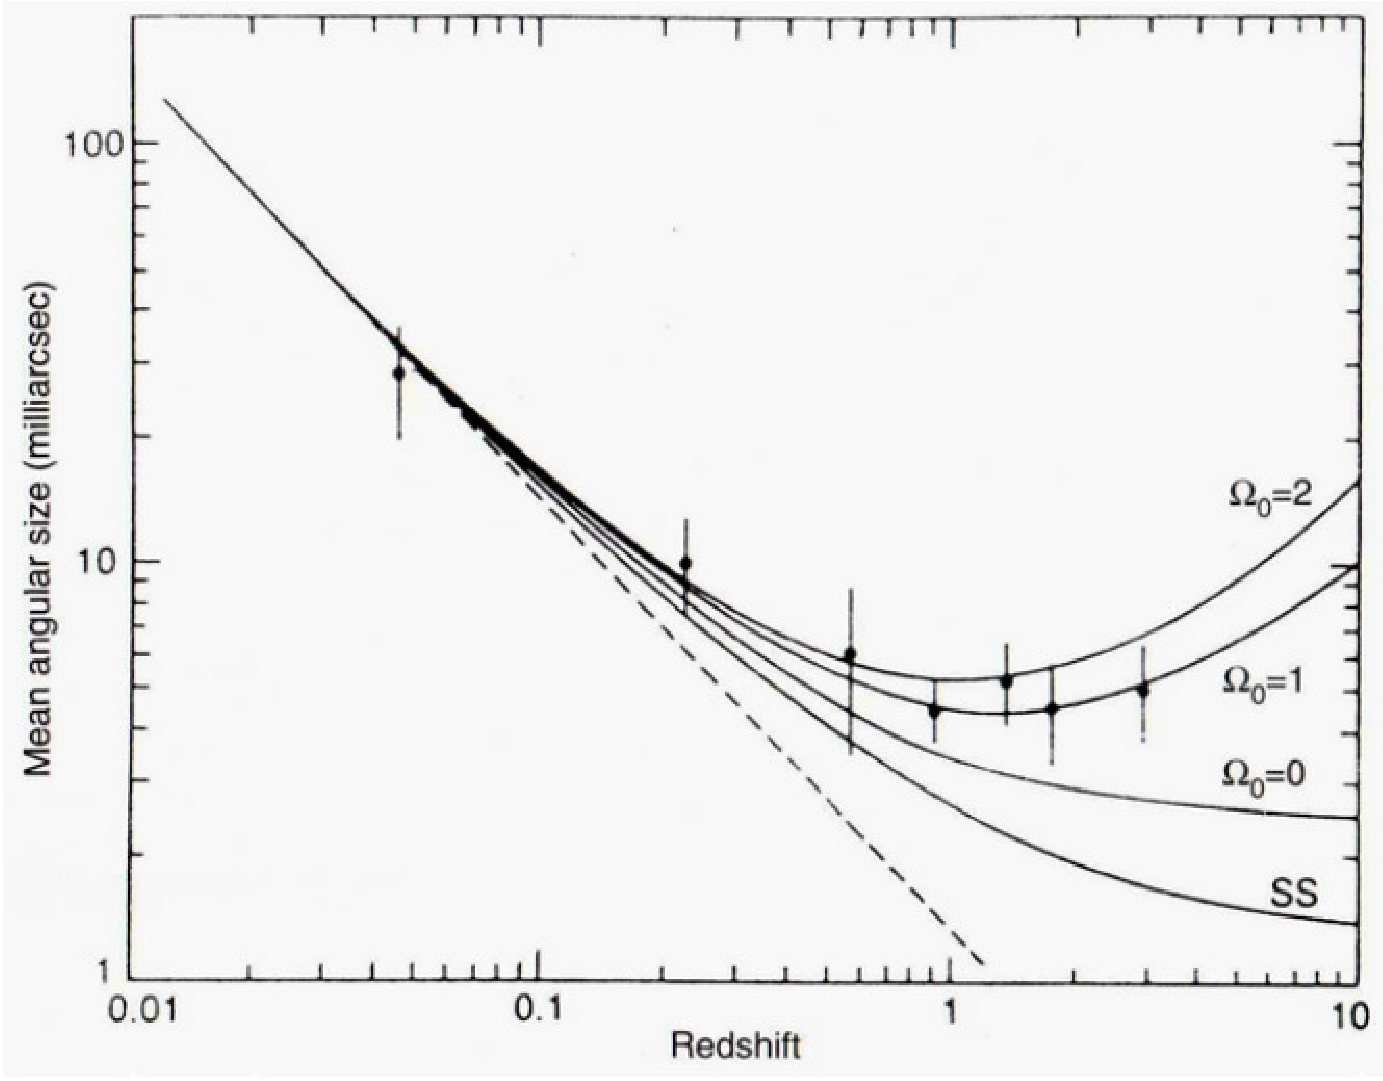
\includegraphics[width=0.8\textwidth]{figure/diametri_angolari_1.pdf}
  \caption{Diametro angolare apparente in funzione del logaritmo di $z$.  Al
    crescere di $q_0$ le curve mostrano un appiattimento a $z \simeq 1$ e quindi
    un aumento del diametro apparente a $z$ più alti}
  \label{diam_angolari_1}
\end{figure}
La lunghezza propria $D$ si calcola dalla metrica RW ponendo $dt=dr=d\phi=0$
\begin{equation}
  D= R(t_1) r_1 \Delta \theta  \implies \Delta \theta = \frac{D} {R(t_1) r_1}
\end{equation}
da cui segue
\begin{equation}
  d_A= R(t_1) r_1.
\end{equation}
Dalle definizioni di $d_L$ in \eqref{dis_lum} e $d_A$ segue
\begin{equation}
  d_A = d_L \left( \frac{R_1}{R_0} \right)^2 = \frac{d_L}{(1+z)^2}
\end{equation}
e quindi usando eq. \eqref{15324}
\begin{equation}
  d_A = \frac { \left[ z q_0 +(q_0-1) (-1+\sqrt{2q_0z+1}) \right] }  {H_0 q^2_0
    (1+z)^2}
  \iff
  \Delta \theta  = D \frac{H_0 q^2_0 (1+z)^2} {\left[ z q_0 +(q_0-1)
      (-1+\sqrt{2q_0z+1}) \right]}
\end{equation}
Qui anticipiamo alcune relazioni che troveremo nel capitolo successivo
\begin{align}
  \Omega_0 &= \frac{\rho_0 }{\rho_c}=2 q_0, \\
  \rho_c   &= \frac{3 H_0^2}{8 \pi G}
\end{align}
La fig.~\ref{diam_angolari_1} illustra l'andamento della dimensione angolare di
una sorgente in funzione di $z$ e la sua dipendenza da $q_0$.  Per $z\ll 1$
l'andamento è quello previsto in un universo Euclideo $\Delta \theta \propto
z^{-1}$ .  All'avvicinarsi a $z=1$ si verifica un appiattimento, e per valori di
$z>1$ una inversione per cui al crescere della distanza (e red-shift) la
dimensione apparente della sorgente cresce.  Tale comportamento, inaspettato in
un universo Euclideo, è dovuto al fatto che per distanze elevate cominciano ad
intervenire effetti di curvatura che modificano le traiettorie dei fotoni
rispetto alla propagazione rettilinea Euclidea.  Poiché la curvatura della
traiettoria di un fotone dipende (a parità di distanza) dalla densità media di
materia gravitante attraversata (che è misurata da $q_0$), vi sarà una
dipendenza di $\Delta \theta$ dai parametri di decelerazione e densità
$\Omega_0$ come mostrato nelle fig.~\ref{diam_angolari_1} \ref{diam_angolari_2}.
Possiamo vedere la cosa come un effetto di ``lente gravitazionale'' operata
dall'intero Universo e il cui effetto è di ingrandire le dimensioni apparenti di
oggetti lontanissimi.
\begin{figure}
  \centering{}
  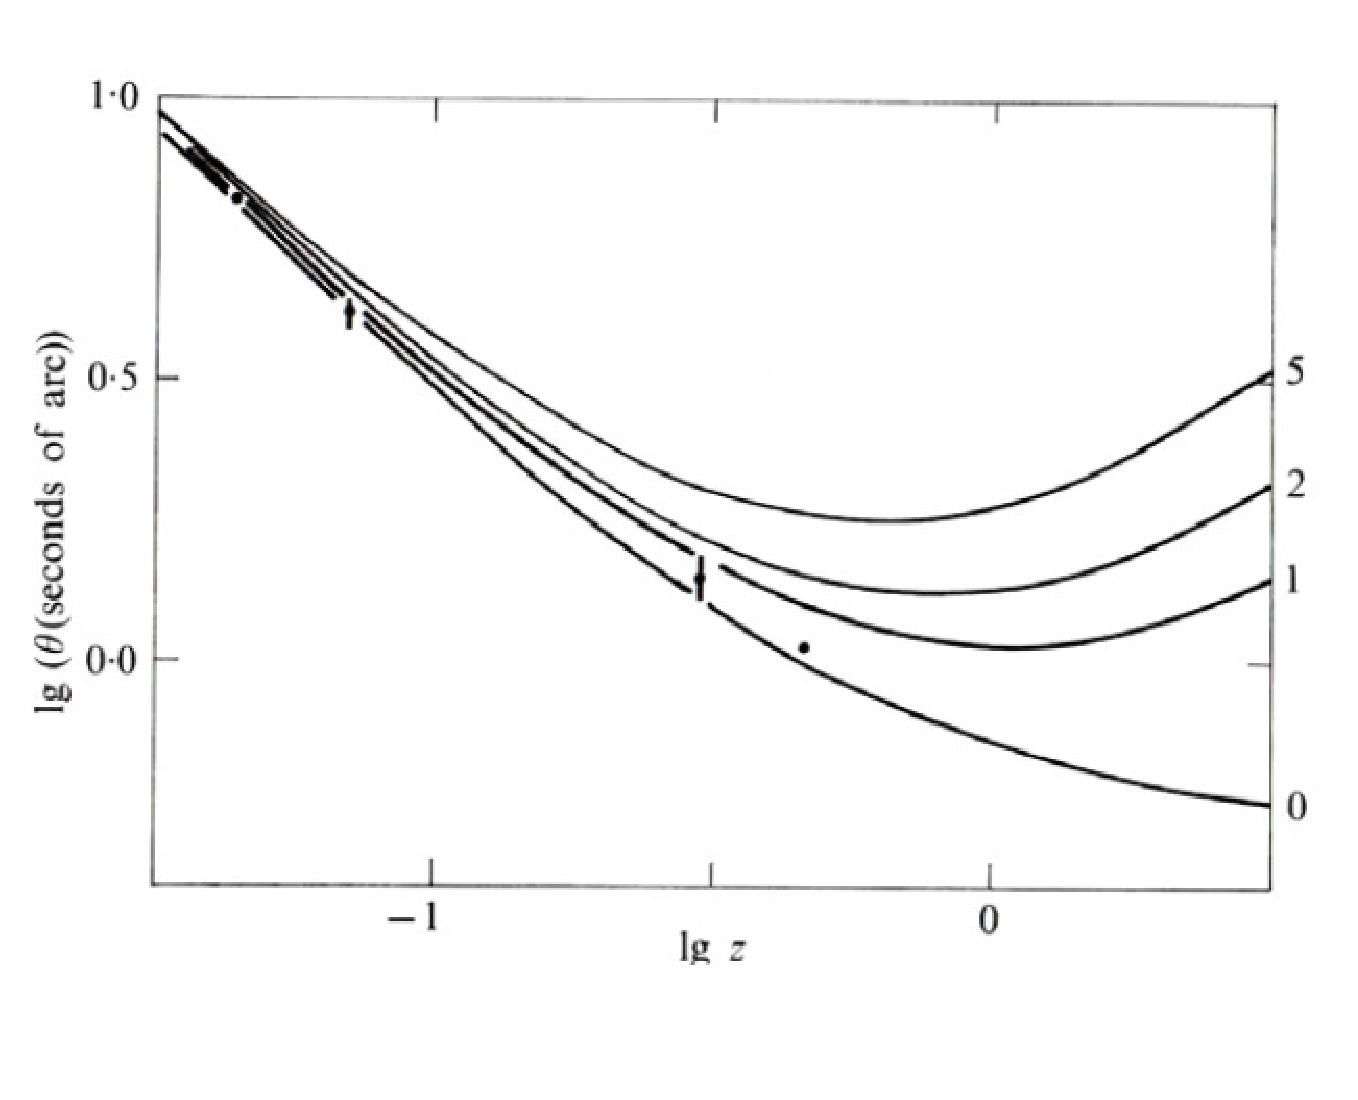
\includegraphics[width=0.75\textwidth]{figure/diametri_angolari_2.pdf}
  \caption{Diametro angolare e parametro di densità $\Omega_0$}
  \label{diam_angolari_2}
\end{figure}
L'utilizzo del test in riferimento alle dimensioni angolari delle radiosorgenti
compatte osservate con il sistema interferometrico ad altissima risoluzione VLBI
è consistente con $q_0=0.5$, come mostrato in fig.~\ref{diam_angolari_2}.

%%% Local Variables:
%%% mode: latex
%%% TeX-master: "../cosmo"
%%% fill-column: 80
%%% End:
